% LuaLaTeX

\documentclass[a4paper, twoside, 12pt]{article}
\usepackage[latin]{babel}
%\usepackage[landscape, left=3cm, right=1.5cm, top=2cm, bottom=1cm]{geometry} % okraje stranky
\usepackage[landscape, a4paper, mag=1166, truedimen, left=2cm, right=1.5cm, top=1.6cm, bottom=0.95cm]{geometry} % okraje stranky

\usepackage{fontspec}
\setmainfont[FeatureFile={junicode.fea}, Ligatures={Common, TeX}, RawFeature=+fixi]{Junicode}
%\setmainfont{Junicode}

% shortcut for Junicode without ligatures (for the Czech texts)
\newfontfamily\nlfont[FeatureFile={junicode.fea}, Ligatures={Common, TeX}, RawFeature=+fixi]{Junicode}

% Hebrew font:
% http://scripts.sil.org/cms/scripts/page.php?site_id=nrsi&id=SILHebrUnic2
\newfontfamily\hebfont[Scale=1]{Ezra SIL}

\usepackage{multicol}
\usepackage{color}
\usepackage{lettrine}
\usepackage{fancyhdr}

% usual packages loading:
\usepackage{luatextra}
\usepackage{graphicx} % support the \includegraphics command and options
\usepackage{gregoriotex} % for gregorio score inclusion
\usepackage{gregoriosyms}
\usepackage{wrapfig} % figures wrapped by the text
\usepackage{parcolumns}
\usepackage[contents={},opacity=1,scale=1,color=black]{background}
\usepackage{tikzpagenodes}
\usepackage{calc}
\usepackage{longtable}
\usetikzlibrary{calc}

\setlength{\headheight}{14.5pt}

% Commands used to produce a typical "Conventus" booklet

\newenvironment{titulusOfficii}{\begin{center}}{\end{center}}
\newcommand{\dies}[1]{#1

}
\newcommand{\nomenFesti}[1]{\textbf{\Large #1}

}
\newcommand{\celebratio}[1]{#1

}

\newcommand{\hora}[1]{%
\vspace{0.5cm}{\large \textbf{#1}}

\fancyhead[LE]{\thepage\ / #1}
\fancyhead[RO]{#1 / \thepage}
\addcontentsline{toc}{subsection}{#1}
}

% larger unit than a hora
\newcommand{\divisio}[1]{%
\begin{center}
{\Large \textsc{#1}}
\end{center}
\fancyhead[CO,CE]{#1}
\addcontentsline{toc}{section}{#1}
}

% a part of a hora, larger than pars
\newcommand{\subhora}[1]{
\begin{center}
{\large \textit{#1}}
\end{center}
%\fancyhead[CO,CE]{#1}
\addcontentsline{toc}{subsubsection}{#1}
}

% rubricated inline text
\newcommand{\rubricatum}[1]{\textit{#1}}

% standalone rubric
\newcommand{\rubrica}[1]{\vspace{3mm}\rubricatum{#1}}

\newcommand{\notitia}[1]{\textcolor{red}{#1}}

\newcommand{\scriptura}[1]{\hfill \small\textit{#1}}

\newcommand{\translatioCantus}[1]{\vspace{1mm}%
{\noindent\footnotesize \nlfont{#1}}}

% pruznejsi varianta nasledujiciho - umoznuje nastavit sirku sloupce
% s prekladem
\newcommand{\psalmusEtTranslatioB}[3]{
  \vspace{0.5cm}
  \begin{parcolumns}[colwidths={2=#3}, nofirstindent=true]{2}
    \colchunk{
      \input{#1}
    }

    \colchunk{
      \vspace{-0.5cm}
      {\footnotesize \nlfont
        \input{#2}
      }
    }
  \end{parcolumns}
}

\newcommand{\psalmusEtTranslatio}[2]{
  \psalmusEtTranslatioB{#1}{#2}{8.5cm}
}


\newcommand{\canticumMagnificatEtTranslatio}[1]{
  \psalmusEtTranslatioB{#1}{temporalia/extra-adventum-vespers/magnificat-boh.tex}{12cm}
}
\newcommand{\canticumBenedictusEtTranslatio}[1]{
  \psalmusEtTranslatioB{#1}{temporalia/extra-adventum-laudes/benedictus-boh.tex}{10.5cm}
}

% volne misto nad antifonami, kam si zpevaci dokresli neumy
\newcommand{\hicSuntNeumae}{\vspace{0.5cm}}

% prepinani mista mezi notovymi osnovami: pro neumovane a neneumovane zpevy
\newcommand{\cantusCumNeumis}{
  \setgrefactor{17}
  \global\advance\grespaceabovelines by 5mm%
}
\newcommand{\cantusSineNeumas}{
  \setgrefactor{17}
  \global\advance\grespaceabovelines by -5mm%
}

% znaky k umisteni nad inicialu zpevu
\newcommand{\superInitialam}[1]{\gresetfirstlineaboveinitial{\small {\textbf{#1}}}{\small {\textbf{#1}}}}

% pars officii, i.e. "oratio", ...
\newcommand{\pars}[1]{\textbf{#1}}

\newenvironment{psalmus}{
  \setlength{\parindent}{0pt}
  \setlength{\parskip}{5pt}
}{
  \setlength{\parindent}{10pt}
  \setlength{\parskip}{10pt}
}

%%%% Prejmenovat na latinske:
\newcommand{\nadpisZalmu}[1]{
  \hspace{2cm}\textbf{#1}\vspace{2mm}%
  \nopagebreak%

}

% mode, score, translation
\newcommand{\antiphona}[3]{%
\hicSuntNeumae
\superInitialam{#1}
\includescore{#2}

#3
}
 % Often used macros
%%%% Preklady jednotlivych zpevu (nektere se opakuji, a je dobre mit je
% vsechny na jedne hromade)

\newcommand{\trOratioAnteOfficium}{\translatioCantus{Otevři, Pane, má ústa, abych chválil tvé svaté jméno.
Očisti mé srdce od všech marnivých, zvrácených a~jiných myšlenek, osvěť rozum, rozněť cit,
abych mohl důstojně, soustředěně a~zbožně recitovat a~vysloužil si být
vyslyšen před tváří tvé velebnosti. Skrze Krista…}}

\newcommand{\trOratioPostOfficium}{\translatioCantus{\textit{Následující modlitbu
opatřil pro ty, kdo ji zbožně vyřknou po hodinkách, zesnulý papež Lev X.
odpustky za hříchy vzniklé při konání hodinek z~lidské křehkosti. Říká se
vkleče.}
Svatosvaté a~nerozdílné Trojici, ukřižovanému lidství našeho Pána Ježíše
Krista, přeblažené a~přeslavné plodné neporušenosti vždy Panny Marie
i~souhrnu všech svatých buď ode všeho stvoření věčná chvála, čest a~sláva, nám
pak buď dáno odpuštění všech hříchů, po nekonečné věky věků. Amen.}}

% HOURS ---

\newcommand{\trAntI}{\translatioCantus{Jasné narození slavné Panny Marie,
z pokolení (dosl. ze semene) Abrahámova, vzešlé z kmene Judova, z rodu Davidova.}}
\newcommand{\trAntII}{\translatioCantus{Dnes je Narození svaté Panny 
Marie, jejíž předrahý život osvěcuje všechny církve.}}

\newcommand{\trAntIII}{\translatioCantus{Maria, jež vzešla 
z královského rodu, září; myslí i duchem ji zbožně prosíme, aby 
nám pomáhala svými přímluvami.}}

\newcommand{\trAntIV}{\translatioCantus{Srdcem i duchem pějme Kristu 
k slávě o této svaté slavnosti vznešené Rodičky Boží Marie.}}

\newcommand{\trAntV}{\translatioCantus{Příjemně \notitia{?} 
oslavujme Narození blahoslavené Marie,
aby se ona za nás přimlouvala u Pána Ježíše Krista.}}

\newcommand{\trCapituli}{\translatioCantus{Před věky, na počátku mě stvořil, potrvám věčně. Ve svatém Stanu jsem před ním konala službu.}}

\newcommand{\trRespVesp}{\translatioCantus{Buď zdráva, Maria,
plná milosti: \grestar{} Pán s tebou. \Vbardot{} Požehnaná jsi mezi ženami,
a požehnaný plod života (ve smyslu lůna, břicha) tvého.}}

\newcommand{\trVersus}{\translatioCantus{\Vbardot{} Dnes je Narození svaté Panny Marie. \Rbardot{} Jejíž předrahý život osvěcuje všechny církve.}}

\newcommand{\trAntMagnificatI}{\translatioCantus{Konejme památku
veledůstojného narození slavné Panny Marie,
jíž se dostalo mateřské důstojnosti bez ztráty panenské cudnosti.}}

% Tento preklad je vice nez nejisty a ani alternativy, ktere jsem
% videl, me nepresvedcily...
\newcommand{\trAntBenedictus}{\translatioCantus{Slavnostně slavme 
dnešní narození Marie, vždy Panny a Rodičky Boží: v něm se objevuje
vysokost trůnu (totiž Marie, trůnu Božího Syna), aleluja.}}

\newcommand{\trAntMagnificatII}{\translatioCantus{Tvé narození,
Bohorodičko Panno, vyhlásilo radost celému světu:
z tebe totiž vzešlo Slunce spravedlnosti, Kristus, náš Bůh:
jenž zrušil kletbu a dal nám požehnání: přemohl smrt a dal nám život věčný.}}

\newcommand{\trOrationis}{\translatioCantus{Prosíme tě, Bože, 
uděl svým služebníkům dar nebeské milosti,
aby těm, jimž slehnutím blahoslavené Panny vyvstal počátek spásy, 
slavnost k poctě jejího narození přinesla
rozhojnění pokoje.
Skrze tvého Syna, našeho Pána Ježíše Krista, který s tebou žije a kraluje,
Bůh, v jednotě Ducha svatého po všechny věky věků.}}

\newcommand{\trFideliumAnimae}{\translatioCantus{\Vbardot{} Duše věrných ať pro
milosrdenství Boží odpočívají v~pokoji. \Rbardot{} Amen.}}

% Completorium

\newcommand{\trJubeDomne}{\translatioCantus{Rač, pane, požehnat.}}

\newcommand{\trComplBenedictio}{\translatioCantus{Pokojnou noc a~svatou smrt
nechť nám dopřeje všemohoucí Pán. \Rbardot{} Amen.}}

\newcommand{\trComplLectioBr}{\translatioCantus{Buďte střízliví, bděte.
Váš protivník Ďábel obchází jako lev řvoucí a~hledá, koho by pohltil.
Postavte se proti němu pevní ve víře.  Ale ty, Pane, smiluj se nad námi.
\Rbardot{} Bohu díky.}}

\newcommand{\trComplAntI}{\translatioCantus{Rač se smilovati nade mnou,
Hospodine, a vyslyš mou modlitbu.}}

\newcommand{\trComplCapituli}{\translatioCantus{Jsi přece, Hospodine,
uprostřed nás a~jmenujeme se po tobě.  Neopouštěj nás, Pane, náš Bože.}}

\newcommand{\trRespCompl}{\translatioCantus{Do tvých rukou, Pane, \grestar{}
poroučím svého ducha. \Vbardot{} Ty mne zachráníš, Pane, Bože věrný.}}

\newcommand{\trComplVersus}{\translatioCantus{\Vbardot{} Střez mne jako zřítelnici oka,
aleluja. \Rbardot{} Ve stínu svých křídel uschovej mne, aleluja.}}

\newcommand{\trAntSalvaNos}{\translatioCantus{Ochraňuj nás, Pane, když
bdíme, a~buď s~námi, když spíme, ať bdíme s~Kristem a~odpočíváme v~pokoji.}}

\newcommand{\trComplOrationis}{\translatioCantus{Zavítej, prosíme, Pane, sem
do našeho příbytku a~daleko od něj zažeň všechny úklady nepřítele. Ať tu
bydlí tví svatí andělé a~tvoje požehnání buď nad ním stále. Skrze…}}

\newcommand{\trSalveRegina}{\translatioCantus{Zdrávas Královno, matko
milosrdenství, živote, sladkosti a naděje naše, buď zdráva!
K tobě voláme, vyhnaní synové Evy,
k tobě vzdycháme, lkajíce a plačíce
v tomto slzavém údolí.
A proto, orodovnice naše,
obrať k nám své milosrdné oči
a Ježíše, požehnaný plod života svého,
nám po tomto putování ukaž,
ó milostivá, ó přívětivá,
ó přesladká, Panno Maria!}}

\newcommand{\trOraProNobis}{\translatioCantus{\Vbardot{} 
Oroduj za nás, svatá Boží Rodičko,
\Rbardot{} aby nám Kristus dal účast na svých zaslíbeních.}}

% Matutinum

\newcommand{\trMatInvitatorium}{\translatioCantus{}}

\newcommand{\trMatVeniteA}{\translatioCantus{Pojďte, chvalme s~radostí Pána,
s~jásotem slavme Boha, svou spásu; předstupme před tvář jeho s~díky, písně plesu pějme jemu.}}

\newcommand{\trMatVeniteB}{\translatioCantus{Neboť Bůh veliký jest Hospodin, a~král nade všecky bohy.
Jsouť v~jeho ruce všecky hlubiny země, temena hor jsou majetek jeho.}}

\newcommand{\trMatVeniteC}{\translatioCantus{Jehoť jest moře, neb on je učinil; i~souš
je dílo jeho rukou. Pojďme, klanějme se, padněme, klekněme před Pánem, svým
tvůrcem. Jeť on Pán, náš Bůh, a~my jsme lid, jejž on vodí a~ovce, jež pase.}}

\newcommand{\trMatVeniteD}{\translatioCantus{Kéž byste poslechli dnes hlasu jeho:
,,Nezatvrzujte svých srdcí jak v~Hádce, jak v~Pokušení na poušti, kde vaši otcové pokoušeli mne,
zkoušeli mne, ač vídali skutky mé.``}}

\newcommand{\trMatVeniteE}{\translatioCantus{Čtyřicet roků mrzel jsem se na to pokolení
a~řekl jsem: ,,Lid je to myslí stále bloudící``! Oni však nechtěli znáti mé cesty, takže jsem
přisáhl ve svém hněvu: ,,Nedojdou odpočinku mého!\mbox{}``}}

\newcommand{\trMatAntI}{\translatioCantus{}}

\newcommand{\trMatAntII}{\translatioCantus{}}

\newcommand{\trMatAntIII}{\translatioCantus{}}

\newcommand{\trMatVersusI}{\translatioCantus{}}

\newcommand{\trMatAbsolutioI}{\translatioCantus{Vyslyš Pane Ježíši Kriste
prosby svých služebníků \gredagger{} a~smiluj se nad námi, \grestar{} jenž
s~Otcem a~Duchem…}}

\newcommand{\trMatBenedictioI}{\translatioCantus{Rač, pane, požehnat.
Věčný Otec nám stále žehnej. \Rbardot{} Amen.}}

\newcommand{\trMatLecI}{\translatioCantus{Kéž by mě zulíbal polibky svých úst. 
Tvé milování je nad víno lahodnější;
vybraně voní tvé voňavky;
rozlévající se olej je tvé jméno,
proto tě dívky milují.
Strhni mě za sebou, poběžme!
Král mě uvedl do svých komnat;
budeš nám radostí a jásotem.
Víc než víno oslavíme tvé milování;
věru po právu jsi milován!
Snědá jsem, a přece krásná, jeruzalémské dcery,
jako stany kedarské,
jako šalmské závěsy.
}}

\newcommand{\trMatRespI}{\translatioCantus{}}

\newcommand{\trMatBenedictioII}{\translatioCantus{Rač, pane, požehnat.
Jednorozený Boží Syn nám žehnej \grestar{} a nám pomáhej. \Rbardot{} Amen.}}

\newcommand{\trMatLecII}{\translatioCantus{Nehleďte na mou osmahlou pleť:
to mě slunce ožehlo.
Synové mé matky se na mne rozzlobili,
poslali mě hlídat vinice.
A svou vinici, tu jsem nehlídala!
Pověz mi tedy, ty, jehož miluje mé srdce:
kam zavedeš své stádo pást,
kde ho necháš za poledne odpočívat?
Abych už nebloudila jako tulačka
poblíž stád druhů tvých.
Nevíš-li to, nejrásnější z žen,
jdi po stopách stáda
a kůzlata svá zaveď, ať se pasou
poblíž obydlí pastýřů.
Ke své klisně zapřažené do vozu faraonova
tebe, mé milá, přirovnávám.
Stále krásné jsou tvé líce s náušnicemi
i tvé hrdlo v náhrdelnících.}}

\newcommand{\trMatRespII}{\translatioCantus{}}

\newcommand{\trMatBenedictioIII}{\translatioCantus{Rač, pane, požehnat.
Milost Ducha Svatého ať osvítí nám smysly \grestar{} i srdce. \Rbardot{} Amen.}}

\newcommand{\trMatLecIII}{\translatioCantus{Zhotovíme ti zlaté náušnice
a kuličky ze stříbra.
Když král stoluje,
vydechuje můj nard svou vůni.
Můj milý je polštářek s myrhou,
jenž mi odpočívá mezi ňadry.
Můj milý je hrozen šáchoru
ve vinicích v Engadi.
Jak jsi krásná, milá moje,
jak jsi krásná!
Tvé oči jsou holubice.
Jak jsi krásný, můj milý,
jak líbezný!
Naše lože je samá zeleň.
Trámoví našeho domu je z cedru,
naše ostění z cypřiše.}}

\newcommand{\trMatRespIII}{\translatioCantus{}}

\newcommand{\trMatAntIV}{\translatioCantus{}}

\newcommand{\trMatAntV}{\translatioCantus{}}

\newcommand{\trMatAntVI}{\translatioCantus{}}

\newcommand{\trMatVersusII}{\translatioCantus{}}

\newcommand{\trMatAbsolutioII}{\translatioCantus{
Tvá milost a laskavost nechť nám pomáhá, jenž žiješ a vládneš s Otcem a Svatým Duchem na věky věků.}}

\newcommand{\trMatBenedictioIV}{\translatioCantus{Rač, pane, požehnat.
Bůh Otec všemohoucí, \grestar{} buď k nám milostivý a odpouštějící. \Rbardot{} Amen.}}

\newcommand{\trMatLecIV}{\translatioCantus{}}

\newcommand{\trMatRespIV}{\translatioCantus{}}

\newcommand{\trMatBenedictioV}{\translatioCantus{}}

\newcommand{\trMatLecV}{\translatioCantus{}}

\newcommand{\trMatRespV}{\translatioCantus{}}

\newcommand{\trMatBenedictioVI}{\translatioCantus{Rač, pane, požehnat.
Bůh rozněť v nás oheň své lásky. \Rbardot{} Amen.}}

\newcommand{\trMatLecVI}{\translatioCantus{}}

\newcommand{\trMatRespVI}{\translatioCantus{}}

\newcommand{\trMatAntVII}{\translatioCantus{}}

\newcommand{\trMatAntVIII}{\translatioCantus{}}

\newcommand{\trMatAntIX}{\translatioCantus{}}

\newcommand{\trMatVersusIII}{\translatioCantus{}}

\newcommand{\trMatAbsolutioIII}{\translatioCantus{Z okovů našich hříchů,
\grestar{} vysvoboď nás všemohoucí a milosrdný Pán. \Rbardot{} Amen.}}

\newcommand{\trMatBenedictioVII}{\translatioCantus{Rač, pane, požehnat.
Čtení evangelia nechť je nám \grestar{} spásou a ochranou. \Rbardot{} Amen.}}

\newcommand{\trMatLecVIIa}{\translatioCantus{
  Rodokmen Ježíše Krista, syna Davidova, syna Abrahámova:
  Abrahám zplodil Izáka,
  Izák zplodil Jakuba.}}

\newcommand{\trMatLecVIIb}{\translatioCantus{}}

\newcommand{\trMatRespVII}{\translatioCantus{}}

\newcommand{\trMatBenedictioVIII}{\translatioCantus{Rač, pane, požehnat.
\Rbardot{} Amen.}}

\newcommand{\trMatLecVIII}{\translatioCantus{}}

\newcommand{\trMatRespVIII}{\translatioCantus{}}

\newcommand{\trMatBenedictioIX}{\translatioCantus{Rač, pane, požehnat.
Do společnosti občanů nebes \grestar{} ať nás dovede král andělů.
\Rbardot{} Amen.}}

\newcommand{\trMatLecIX}{\translatioCantus{}}

% from the Czech Liturgia horarum
\newcommand{\trTeDeum}{\begin{translatioMulticol}{3}

Bože, tebe chválíme, 
tebe, Pane, velebíme.

Tebe, věčný Otče, 
oslavuje celá země.

Všichni andělé, 
cherubové i~serafové,

všechny mocné nebeské zástupy 
bez ustání volají:

Svatý, Svatý, Svatý, 
Pán, Bůh zástupů.

Plná jsou nebesa i~země 
tvé vznešené slávy.

Oslavuje tě 
sbor tvých apoštolů,

chválí tě 
velký počet proroků,

vydává o~tobě svědectví 
zástup mučedníků;

a~po celém světě 
vyznává tě tvá církev:

neskonale velebný, 
všemohoucí Otče,

úctyhodný Synu Boží, 
pravý a~jediný,

božský Utěšiteli, 
Duchu svatý.

Kriste, Králi slávy, 
tys od věků Syn Boha Otce;

abys člověka vykoupil, 
stal ses člověkem a~narodil ses z~Panny;

zlomil jsi osten smrti 
a~otevřel věřícím nebe;

sedíš po Otcově pravici 
a~máš účast na jeho slávě.

Věříme, že přijdeš soudit, 

a~proto tě prosíme:
přispěj na pomoc svým služebníkům, 
vždyť jsi je vykoupil svou předrahou krví;

dej, ať se radují s~tvými svatými 
ve věčné slávě.

Zachraň, Pane, svůj lid, žehnej svému dědictví, 
veď ho a~stále pozvedej.

Každý den tě budeme velebit 
a~chválit tvé jméno po všechny věky.

Pomáhej nám i~dnes, 
ať se nedostaneme do područí hříchu.

Smiluj se nad námi, Pane, 
smiluj se nad námi.

Ať spočine na nás tvé milosrdenství, 
jak doufáme v~tebe.

Pane, k~tobě se utíkáme, 
ať nejsme zahanbeni na věky. 
\end{translatioMulticol}}

\newcommand{\trMatEvangelium}{\translatioCantus{
  Rodokmen Ježíše Krista, syna Davidova, syna Abrahámova:
  Abrahám zplodil Izáka,
  Izák zplodil Jakuba,
  Jakub zplodil Judu a jeho bratry,
  Juda zplodil Farese a Zaru z Tamary,
  Fares zplodil Esroma,
  Esrom zplodil Arama,
  Aram zplodil Aminadaba,
  Aminadab zplodil Naasona,
  Naason zplodil Salmona,
  Salmon zplodil Boaze z Rahaby,
  Boaz zplodil Jobeda z Rut,
  Jobed zplodil Jessea,
  Jesse zplodil krále Davida.
  David zplodil Šalomouna z Uriášovy ženy,
  Šalomoun zplodil Roboama,
  Roboam zplodil Abiu,
  Abia zplodil Asu,
  Asa zplodil Josafata,
  Josafat zplodil Jorama,
  Joram zplodil Oziáše,
  Oziáš zplodil Joatama,
  Joatam zplodil Achaze,
  Achaz zplodil Ezechiáše,
  Ezechiáš zplodil Manasesa,
  Manases zplodil Amona,
  Amon zplodil Josiáše,
  Josiáš zplodil Jechoniáše a jeho bratry;
  tehdy došlo k odvlečení do Babylonu.
  Po odvlečení do Babylonu:
  Jechoniáš zplodil Salatiela,
  Salatiel zplodil Zorobabela,
  Zorobabel zplodil Abiuda,
  Abiud zplodil Eljakima,
  Eljakim zplodil Azora,
  Ator zplodil Sadoka,
  Sadok zplodil Achima,
  Achim zplodil Eliuda,
  Eliud zplodil Eleazara,
  Eleatar zplodil Matana,
  Matan zplodil Jakuba,
  Jakub zplodil Josefa, manžela Marie,
  z níž se narodil Ježíš, který se nazývá Kristus.}}

\newcommand{\trTeDecetLaus}{\translatioCantus{Tobě chvála, Tobě zpěvy, Tobě
sláva, Bohu Otci i~Synu i~Svatému Duchu, na věky věků. \Rbardot{} Amen.}}

% MASS ---

\newcommand{\trIntroitus}{\translatioCantus{Radujme se všichni
v Pánu, slavíce svátek ke cti Panny Marie: z něj se radují andělé
a spoluchválí Božího Syna. \textit{\color{red}Žl.} Má ústa vydala dobré slovo,
přednáším svá díla králi.}}

\newcommand{\trGraduale}{\translatioCantus{Požehnaná a ctihodná jsi,
Panno Maria: nedotčená (co do panenství) jsi byla shledána matkou
Spasitele. \Vbardot{} Panno Boží Rodičko, ten, jehož nepojme ani celý svět,
se uzavřel do tvých útrob, když se stal člověkem.}}

\newcommand{\trAlleluia}{\translatioCantus{Aleluja. \Vbardot{} Skvělá slavnost
slavné Panny Marie, z pokolení (dosl. ze semene) Abrahámova, vzešlé z kmene 
Judova, z rodu Davidova.}}

\newcommand{\trOffertorium}{\translatioCantus{Blažená jsi, Panno Maria,
tys nosila Stvořitele všeho; porodila jsi toho, který tě utvořil,
a na věky zůstáváš Pannou.}}

\newcommand{\trCommunio}{\translatioCantus{Budou mě blahoslavit
všechna pokolení, protože mi učinil veliké věci ten, který je mocný.}}

% LITTLE HOURS ---

\newcommand{\trVersusTertia}{\translatioCantus{\Vbardot{} \Rbardot{}}}

\newcommand{\trCapituliEtSic}{\translatioCantus{
Tak jsem se usadila na Sionu a v milovaném městě jsem nalezla odpočinek,
v Jeruzalémě vykonávám svou moc.
Zakořenila jsem u lidu plného slývy, na panství Páně, v jeho dědictví.}}

\newcommand{\trVersusSexta}{\translatioCantus{\Vbardot{} \Rbardot{}}}

\newcommand{\trCapituliInPlateis}{\translatioCantus{
Na planině jako skořicovník a akant jsem vydávala vůni, jako vybraná myrha
jsem voněla.}}

\newcommand{\trVersusNona}{\translatioCantus{\Vbardot{} \Rbardot{}}}
 % Czech translations of the proper texts

\newcommand{\annusEditionis}{2018}

\def\hebinitial#1{%
\leavevmode{\newbox\hebbox\setbox\hebbox\hbox{\hebfont{#1}\hskip 1mm}\kern -\wd\hebbox\hbox{\hebfont{#1}\hskip 1mm}}%
}

%%%% Vicekrat opakovane kousky

\newcommand{\anteOrationem}{
  \rubrica{Ante Orationem, cantatur a Superiore:}

  \pars{Supplicatio Litaniæ.}

  \cuminitiali{}{temporalia/supplicatiolitaniae.gtex}

  \pars{Oratio Dominica.}

  \cuminitiali{}{temporalia/oratiodominica.gtex}

  \rubrica{Deinde dicitur ab Hebdomadario:}

  \cuminitiali{}{temporalia/dominusvobiscum-solemnis.gtex}

  \rubrica{In choro monialium loco Dominus vobiscum dicitur:}

  \sineinitiali{temporalia/domineexaudi.gtex}
}

\setlength{\columnsep}{30pt} % prostor mezi sloupci

%%%%%%%%%%%%%%%%%%%%%%%%%%%%%%%%%%%%%%%%%%%%%%%%%%%%%%%%%%%%%%%%%%%%%%%%%%%%%%%%%%%%%%%%%%%%%%%%%%%%%%%%%%%%%
\begin{document}

% Here we set the space around the initial.
% Please report to http://home.gna.org/gregorio/gregoriotex/details for more details and options
\grechangedim{afterinitialshift}{2.2mm}{scalable}
\grechangedim{beforeinitialshift}{2.2mm}{scalable}

\grechangedim{interwordspacetext}{0.22 cm plus 0.15 cm minus 0.05 cm}{scalable}%
\grechangedim{annotationraise}{-2mm}{scalable}

% Here we set the initial font. Change 38 if you want a bigger initial.
% Emit the initials in red.
\grechangestyle{initial}{\color{red}\fontsize{38}{38}\selectfont}

\pagestyle{empty}

%%%% Titulni stranka
\begin{titulusOfficii}
%\dies{Die 16. Octobris.}
\nomenFesti{Officium Defunctorum}

et

\nomenFesti{Commemoratione Omnium Fidelium Defunctorum}
\celebratio{Duplex.}
\end{titulusOfficii}

% graphic
\vspace{1.5cm}
\begin{center}
%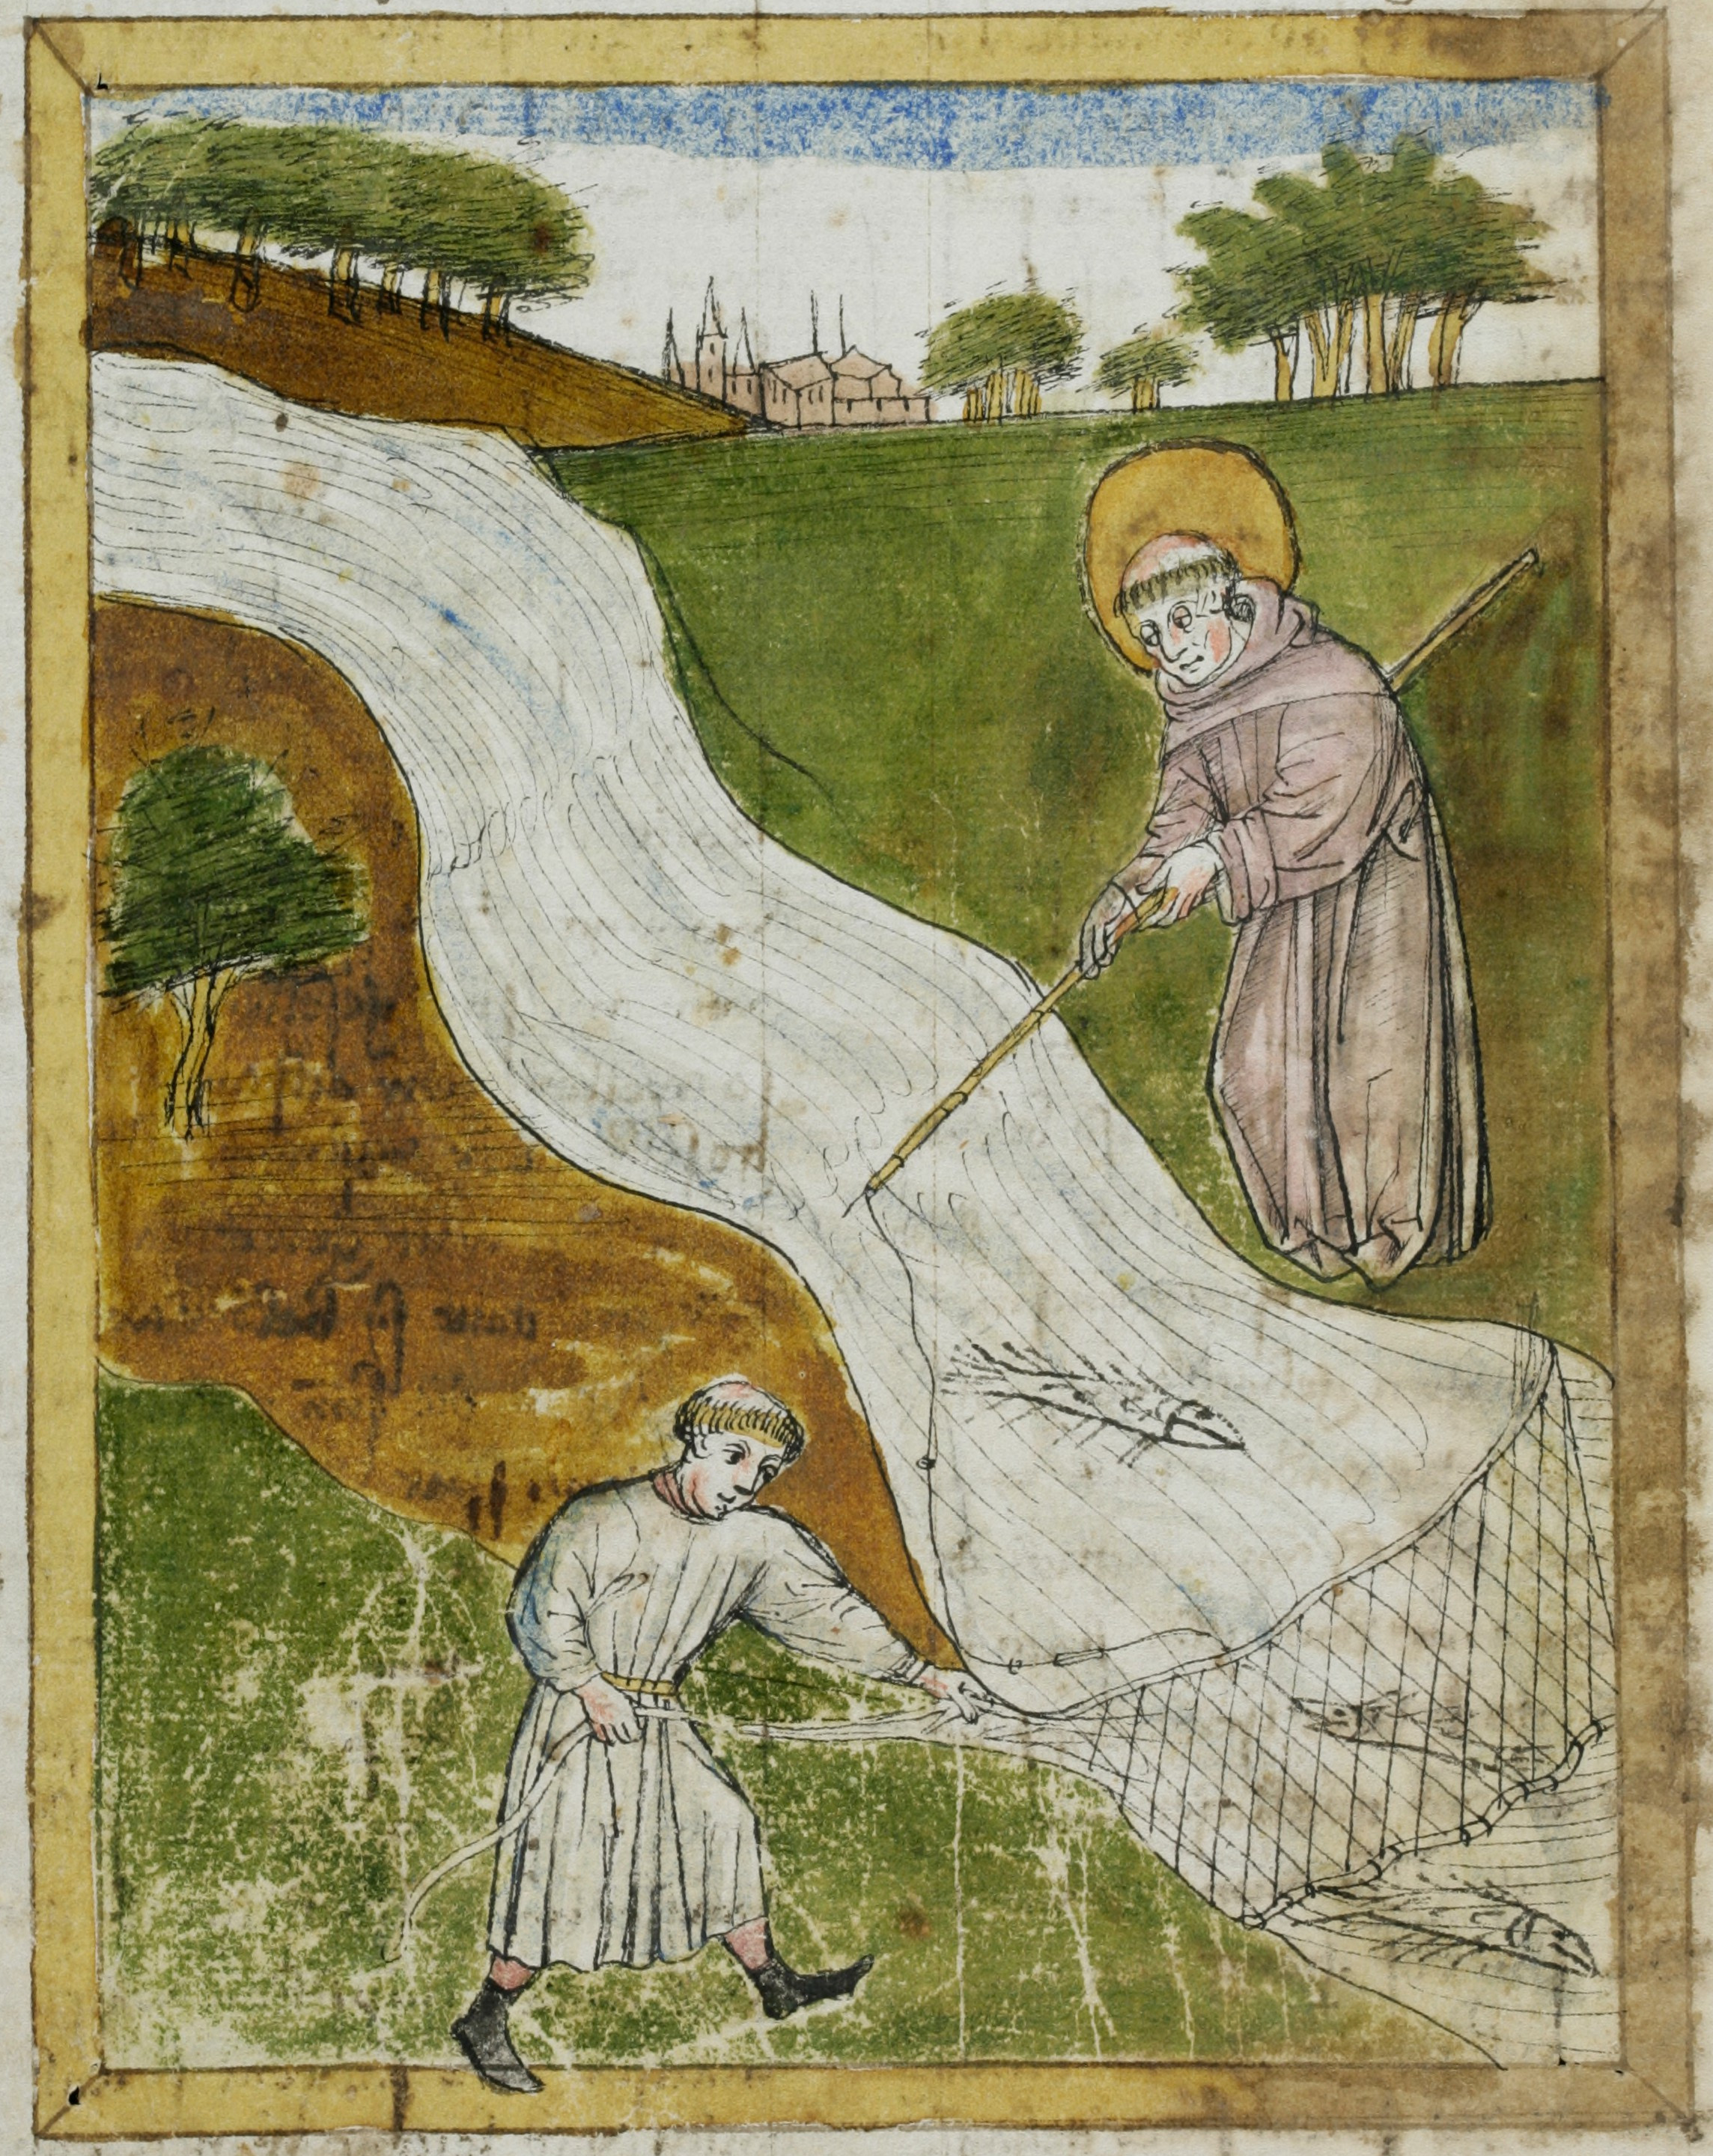
\includegraphics[width=8cm]{gallus2.jpg}
\end{center}

\vfill

\begin{center}
Ad usum et secundum consuetudines chori \guillemotright Conventus Choralis\guillemotleft.

Editio Sancti Wolfgangi \annusEditionis
\end{center}

\pagebreak

\renewcommand{\headrulewidth}{0pt} % no horiz. rule at the header
\fancyhf{}
\pagestyle{fancy}

\pars{Oratio ante divinum Officium.}

\lettrine{{\color{red}A}}{peri,} Dómine, os meum ad benedicéndum nomen sanctum tuum:
munda quoque cor meum ab ómnibus vanis, pervérsis, et aliénis
cogitatiónibus:
intelléctum illúmina, afféctum inflámma,
ut digne, atténte ac devóte hoc Offícium recitáre váleam,
et exaudíri mérear ante conspéctum Divínæ Maiestátis tuæ.
Per Christum, Dóminum nostrum.
\Rbardot{} Amen.

Dómine, in unióne illíus divínæ intentiónis,
qua ipse in terris laudes Deo persolvísti,
has tibi Horas \rubricatum{(vel \textnormal{hanc tibi Horam})} persólvo.

\trOratioAnteOfficium

\vfill

\pars{Oratio post divinum Officium.}

\rubrica{
  Orationem sequentem devote post Officium recitantibus
  Leo Papa X. defectus, et culpas in eo persolvendo ex humana
  fragilitate contractas, indulsit, et dicitur flexis genibus.
}

\lettrine{{\color{red}S}}{acrosánctæ} et indivíduæ Trinitáti,
crucifíxi Dómini nostri Iesu Christi humanitáti,
beatíssimæ et gloriosíssimæ sempérque Vírginis Maríæ
fecúndæ integritáti,
et ómnium Sanctórum universitáti
sit sempitérna laus, honor, virtus et glória
ab omni creatúra,
nobísque remíssio ómnium peccatórum,
per infiníta sǽcula sæculórum.
\Rbardot{} Amen.

\noindent \Vbardot{} Beáta víscera Maríæ Vírginis, quæ portavérunt
ætérni Patris Fílium.\\
\Rbardot{} Et beáta úbera, quæ lactavérunt Christum Dóminum.

\rubrica{Et dicitur secreto \textnormal{Pater noster.} et \textnormal{Ave María.}}

\trOratioPostOfficium

\vfill

\rubrica{In die depositionis, in die post acceptum mortis nuntium, et tertio,
septimo, trigesimo, et anniversario, etiam late sumpto, et quoties
solemniter celebratur Officium, duplicantur Antiphonæ.  In fine vero omnium
Psalmorum semper dicitur: \textnormal{Réquiem ætérnam \grestar{} dona eis
Dómine. Et lux perpétua \grestar{} lůceat eis}; etiam si pro uno tantum fiat
Officium. (Psalmi incipiuntur ut infra notatur, etiam quando non duplicantur
Antiphonæ).}

\vfill

\hora{Ad Vesperas.} %%%%%%%%%%%%%%%%%%%%%%%%%%%%%%%%%%%%%%%%%%%%%%%%%%%%%
\sideThumbs{Vesperæ}

\rubrica{Quoties Vesperæ vel delationem cadaveris ad ecclesiam ac
Responsorium \textnormal{Subveníte}, vel Officium diei currentis immediate
non sequantur, dicitur secreto \textnormal{Pater} et \textnormal{Ave}; secus
absolute incipitur ab Antiphona.}

\vfill
\pagebreak

\cantusCumNeumis

\pars{Psalmus 1.} \scriptura{Ps. 114, 9; \textbf{H390}}

\vspace{-5mm}

\antiphona{III b}{temporalia/vesp-ant1.gtex}

\trVespAntI

\scriptura{Ps. 114}

\initiumpsalmi{temporalia/ps114-initium-iii-b-auto.gtex}

\psalmusEtTranslatioT{temporalia/ps114-comb.tex}{10cm}

%\antiphona{}{temporalia/vesp-ant1.gtex} % repeat the antiphon - new page

\vfill
\pagebreak

\pars{Psalmus 2.} \scriptura{Ps. 119, 5; \textbf{H394}}

\vspace{-5mm}

\antiphona{II D}{temporalia/vesp-ant2.gtex}

\trVespAntII

\vspace{-2mm}

\scriptura{Ps. 119}

\initiumpsalmi{temporalia/ps119-initium-ii-D-auto.gtex}

\vspace{-2mm}

\psalmusEtTranslatioT{temporalia/ps119-comb.tex}{9cm}

%\antiphona{}{temporalia/vesp-ant2.gtex} % repeat the antiphon - new page

\vfill
\pagebreak

\pars{Psalmus 3.} \scriptura{Ps. 120, 7; \textbf{H394}}

\vspace{-5mm}

\antiphona{VIII G\textsuperscript{2}}{temporalia/vesp-ant3.gtex}

\trVespAntIII

\scriptura{Ps. 120}

\initiumpsalmi{temporalia/ps120-initium-viii-G2-auto.gtex}
\psalmusEtTranslatioT{temporalia/ps120-comb.tex}{10cm}

%\antiphona{}{temporalia/vesp-ant3.gtex} % repeat the antiphon - new page

\vfill
\pagebreak

\pars{Psalmus 4.} \scriptura{Ps. 129, 3; \textbf{H394}}

\vspace{-5mm}

\antiphona{VIII G}{temporalia/vesp-ant4.gtex}

\trVespAntIV

\scriptura{Ps. 129}

\initiumpsalmi{temporalia/ps129-initium-viii-G-auto.gtex}
\psalmusEtTranslatioT{temporalia/ps129-comb.tex}{10cm}

%\antiphona{}{temporalia/vesp-ant4.gtex} % repeat the antiphon - new page

\vfill
\pagebreak

\pars{Psalmus 5.} \scriptura{Ps. 137, 8; \textbf{H394}}

\vspace{-5mm}

\antiphona{II D}{temporalia/vesp-ant5.gtex}

\trVespAntV

\scriptura{Ps. 137}

\initiumpsalmi{temporalia/ps137-initium-ii-D-auto.gtex}
\psalmusEtTranslatioT{temporalia/ps137-comb.tex}{10cm}

%\antiphona{}{temporalia/vesp-ant5.gtex} % repeat the antiphon - new page

\vfill
\pagebreak

% Capitulum. %%%
\cantusSineNeumas

\pars{Versus (in loco Capituli).} \scriptura{Ap. 14, 13}

% Versus. %%%
\sineinitiali{temporalia/versus-audivi.gtex}

\noindent \trVersusAudivi

\vfill
\vspace{2mm}
%\pagebreak

\cantusCumNeumis

\pars{Canticum B. Mariæ V.} \scriptura{Io. 6, 37; \textbf{H393}}

\vspace{-5mm}

\antiphona{VII c}{temporalia/vesp-ant-magn.gtex}

\trAntMagnificat

\vspace{-5mm}

\scriptura{Lc. 1, 46-55}

\cantusSineNeumas
\initiumpsalmi{temporalia/magnificat-initium-vii-c.gtex}

\vspace{-6mm}

\psalmusEtTranslatioT{temporalia/magnificat-comb.tex}{10.3cm}

%\antiphona{}{temporalia/vesp-ant-magn.gtex} % repeat the antiphon - new page

\vfill
\pagebreak

\rubrica{Preces infrascriptæ dicuntur flexis genibus, similiter et ad Laudes.}

\vspace{2mm}

\pars{Supplicatio Litaniæ.}

\cuminitiali{}{temporalia/supplicatiolitaniae.gtex}

\vspace{2mm}

\pars{Oratio Dominica.}

\cuminitiali{}{temporalia/oratiodominica.gtex}

\vfill
\pagebreak

\pars{Psalmus 6.}

\rubrica{Sequens Psalmus \textnormal{Lauda ánima mea.} non dicitur in die
obitus seu depositionis defuncti, neque quandocumque Officium recitatur ritu
duplici.}

\scriptura{Ps. 145}

\initiumpsalmi{temporalia/ps145-initium-dir-auto.gtex}
\psalmusEtTranslatioT{temporalia/ps145-comb.tex}{10cm}

\vfill
\pagebreak

\label{oratio}

\rubrica{Deinde:}

\noindent \Vbardot{} A porta ínferi. \Rbardot{} Erue ánimam eius {\color{red}(}ánimas eórum{\color{red})}.

\noindent \Vbardot{} Requiéscat in pace {\color{red}(}Requiéscant in pace{\color{red})}. \Rbardot{} Amen.

\noindent \Vbardot{} Dómine exáudi oratiónem meam. \Rbardot{} Et clamor meus ad te véniat.

\noindent \Vbardot{} Dóminus vobíscum. \Rbardot{} Et cum spíritu tuo.

\vspace{2mm}

\pars{Oratio}

\grechangedim{spaceabovelines}{2mm}{scalable}
\cuminitiali{}{temporalia/oratio.gtex}
\grechangedim{spaceabovelines}{0cm}{scalable}

\rubrica{Dicitur Oratio conveniens ex iis quæ sequuntus; deinde \Vbardot{}
\textnormal{Réquiem ætérnam.} cum reliquis, ut infra.}

\vspace{2mm}

\pars{In die Commemorationis Omnium Fidelium Defunctorum.}

\rubrica{Oratio.}

\lettrine{{\color{red}F}}{idélium} Deus ómnium Cónditor et Redémptor, animábus famulórum famularúmque tuárum remissiónem cunctórum tríbue pecca\textbf{tó}rum:~\gredagger{}
ut indulgéntiam, quam semper \textit{opta}\textbf{vé}runt,~\grestar{}
piis supplicatiónibus conse\textbf{quán}tur. Qui vivis.

\vspace{2mm}

\pars{In die depositionis Defuncti.}

\rubrica{Oratio.}

\lettrine{{\color{red}A}}{bsólve}, quǽsumus Dómine, ánimam fámuli tui {\color{red}N.} {\color{red}(}fámulæ tuæ {\color{red}N.}{\color{red})} ut defúnctus{\color{red}(}a{\color{red})} sǽculo tibi \textbf{vi}vat:~\gredagger{}
et quæ per fragilitátem carnis humána conversatió\textit{ne} \textit{com}\textbf{mí}sit, tu~\grestar{}
vénia misericordíssimæ pietátis abs\textbf{tér}ge. Per Dóminum.

\rubrica{Si autem sit præsens Defuncti cadaver, dicitur sequens Oratio:}

\lettrine{{\color{red}D}}{eus}, cui próprium est miseréri semper et párcere, te súpplices exorámus pro ánima fámuli tui {\color{red}N.} {\color{red}(}fámulæ tuæ {\color{red}N.}{\color{red})} quam hódie de hoc sǽculo migráre ius\textbf{sís}ti:~\gredagger{}
ut non tradas eam in manus inimíci, neque obliviscáris in finem, se iúbeas eam a sansctis Angelis súscipi, et ad pátriam paradí\textit{si} \textit{per}\textbf{dú}ci;~\grestar{}
ut quia in te sperávit et crédidit, non pœ́nas inférni sustíneat, sed gáudia ætérna pos\textbf{sí}deat. Per Dóminum.

%\vspace{2mm}
\vfill
\pagebreak

\pars{In die tertio, septimo et trigesimo depositionis Defuncti.}

\rubrica{Oratio.}

\lettrine{{\color{red}Q}}{uǽsumus} Dómine, ut ánimæ fámuli tui {\color{red}N.} {\color{red}(}fámulæ tuæ {\color{red}N.}{\color{red})} cuius depositiónis diem tértium {\color{red}(\textit{vel}} séptimum, {\color{red}\textit{vel}} trigésimum{\color{red})}, commemo\textbf{rá}mus,~\gredagger{}
Sanctórum atque electórum tuórum largíri digné\textit{ris} \textit{con}\textbf{sór}tium;~\grestar{}
et rorem misericórdiæ tuæ perénnem in\textbf{fún}das. Per Dóminum.

\vspace{2mm}

\pars{In Anniversario.}

\rubrica{Oratio.}

\lettrine{{\color{red}D}}{eus} indulgentiárum \textbf{Dó}mine:~\gredagger{}
da ánimæ fámuli tui {\color{red}N.} {\color{red}(}fámulæ tuæ {\color{red}N. \textit{vel}} animábus famulórum famularúmque tuárum{\color{red})}, cuius {\color{red}(}quorum{\color{red})} anniversárium depositiónis diem com\textit{memo}\textbf{rá}mus,~\grestar{}
refrigérii sedem, quiétis beatitúdinem, et lúminis clari\textbf{tá}tem. Per Dóminum.

\vspace{2mm}

\pars{Pro Summo Pontifice defuncto.}

\rubrica{Oratio.}

\lettrine{{\color{red}D}}{eus}, qui inter summos sacerdótes fámulum tuum {\color{red}N.} ineffábili tua dispositióne connumerári volu\textbf{ís}ti:~\gredagger{}
præsta, quǽsumus; ut qui unigéniti Fílii tui vices in ter\textit{ris} \textit{ge}\textbf{ré}bat,~\grestar{}
sanctórum tuórum pontíficum consórtio perpétuo aggre\textbf{gé}tur. Per eúmdem Dóminum.

\vspace{2mm}

\pars{Pro defuncto Episcopo.}

\rubrica{Oratio.}

\lettrine{{\color{red}D}}{eus}, qui inter apostólicos sacerdótes fámulum tuum {\color{red}N.} {\color{red}(}fámulos tuos tuos {\color{red}N.} et {\color{red}N.}{\color{red})} pontificáli fecísti dignitáte vi\textbf{gé}re:~\gredagger{}
\textit{præsta}, \textbf{quǽ}sumus;~\grestar{}
ut eórum quoque perpétuo aggregé{\color{red}(}n{\color{red})}tur con\textbf{sór}tio. Per Dóminum.

\noindent \textit{Pro Episcopo Cardinali defuncto dicatur:} fámulum tuum {\color{red}N.} Epíscopum Cardinálem pontificáli fecísti dignitáte.

\noindent \textit{Pro Presbytero Cardinali (Episcopo) defuncto:} fámulum tuum {\color{red}N.} Presbýterum Cardinálem pontificáli fecísti.

\noindent \textit{Pro Presbytero (vel Diacono) Cardinali (Sacerdote) defuncto:} fámulum tuum {\color{red}N.} Presbýterum {\color{red}(}Diáconum{\color{red})} Cardinálem sacerdotáli fecísti.

\noindent \textit{Pro Diacono autem Cardinali, qui in ordine Presbyteratus no fuerit constitutus, dicatur Oratio} Inclína Dómine. \textit{quæ habetur paulo infra hoc modo:} ut ánimam fámuli tui {\color{red}N.} Diáconi Cardinális, quam de hoc sǽculo. \textit{etc.}

%\vspace{2mm}
\vfill
\pagebreak

\pars{Pro defuncto Sacerdote.}

\rubrica{Oratio.}

\lettrine{{\color{red}D}}{eus}, qui inter apostólicos sacerdótes fámulum tuum {\color{red}N.} {\color{red}(}fámulos tuos {\color{red}N.} et {\color{red}N.}{\color{red})} sacerdotáli fecísti dignitáte vi\textbf{gé}re:~\gredagger{}
\textit{præsta}, \textbf{quǽ}sumus;~\grestar{}
ut eórum quoque perpétuo aggregé{\color{red}(}n{\color{red})}tur con\textbf{sór}tio. Per Dóminum.

\rubrica{Vel alia Oratio.}

\lettrine{{\color{red}P}}{ræsta}, quǽsumus \textbf{Dó}mine:~\gredagger{}
ut ánima fámuli tui {\color{red}N.} Sacerdótis, quem in hoc sǽculo commorántem, sacris munéribus \textit{deco}\textbf{rás}ti,~\grestar{}
in cælésti sede gloriósa semper ex\textbf{súl}tet. Per Dóminum.

\vspace{2mm}

\pars{Pro uno Defuncto.}

\rubrica{Oratio.}

\lettrine{{\color{red}I}}{nclína} Dómine aurem tuam ad preces nostras, quibus misericórdiam tuam súpplices depre\textbf{cá}mur:~\gredagger{}
ut ánimam fámuli tui {\color{red}N.}, quam de hoc sǽculo migráre iussísti, in pacis ac lucis regió\textit{ne} \textit{con}stítuas,~\grestar{}
et Sanctórum tuórum iúbeas esse con\textbf{sór}tem. Per Dóminum.

\vspace{2mm}

\pars{Pro una Defuncta.}

\rubrica{Oratio.}

\lettrine{{\color{red}Q}}{uǽsumus} Dómine, pro tua pietáte miserére ánimæ fámulæ tuæ {\color{red}N.}:~\gredagger{}
et a contágiis mortalitá\textit{tis} \textit{ex}\textbf{ú}tam,~\grestar{}
in ætérnæ salvatiónis partem re\textbf{stí}tuæ. Per Dóminum.

\vspace{2mm}

\pars{Pro defunctis Fratribus, Propinquis et Benefactoribus.}

\rubrica{Oratio.}

\lettrine{{\color{red}D}}{eus} véniæ largítor et humánæ salútis a\textbf{má}tor:~\gredagger{}
quǽsumus cleméntiam tuam; ut nostræ congregatiónis fratres, propínquos et benefactóres, qui ex hoc sǽculo \textit{transi}\textbf{é}runt,~\grestar{}
beáta María semper Vírgine intercedénte cum ómnibus Sanctis tuis, ad perpétuæ beatitúdinis consórtium perveníre con\textbf{cé}das. Per Dóminum.

%\vspace{2mm}
\vfill
\pagebreak

\pars{Pro pluribus Defunctis.}

\rubrica{Oratio.}

\lettrine{{\color{red}D}}{eus}, cui próprium est miseréri semper et \textbf{pár}cere:~\gredagger{}
propitiáre animábus famulórum famularúmque tuárum, et ómnia eórum peccá\textit{ta} \textit{di}\textbf{mít}te;~\grestar{}
ut mortalitátis vínculis absolútæ, transíre mereántur ad \textbf{vi}tam. Per Dóminum.

\rubrica{Vel alia Oratio.}

\lettrine{{\color{red}A}}{nimábus}, quǽsumus Dómine, famulórum famularúmque tuárum misericórdiam concéde per\textbf{pé}tuam:~\gredagger{}
ut eis profíciat \textit{in} \textit{æ}\textbf{tér}num,~\grestar{}
quod in te speravérunt et credi\textbf{dé}runt. Per Dóminum.

\vspace{2mm}

\pars{Pro patre et matre.}

\pars{Oratio.}

\lettrine{{\color{red}D}}{eus}, qui nos patrem et matrem honoráre præce\textbf{pís}ti:~\gredagger{}
miserére cleménter animábus patris et matris meæ, eorúmque peccá\textit{ta} \textit{di}\textbf{mít}te;~\grestar{}
meque eos in ætérnæ claritátis gáudio fac vi\textbf{dé}re. Per Dóminum.

\noindent \textit{Si fit pro pluribus, dicatur} animábus paréntum nostrórum, \textit{et ubi dicitur} meque, \textit{dicatur} nosque.

\noindent \textit{Si pro patre tantum, dicatur} ánimæ patris mei, \textit{vel} nostri.

\noindent \textit{Si pro matre tantum, dicatur} ánimæ matris meæ, \textit{vel} nostræ.

\vspace{2mm}

\rubrica{Post Orationem dicitur (semper plurali numero):}

\noindent \Vbardot{} Réquiem ætérnam dona eis Dómine. \Rbardot{} Et lux perpétua lúceat eis.

\vspace{1cm}
\rubrica{Deinde Cantores:}
\vspace{2mm}

\sineinitiali{temporalia/requiescant.gtex}

\vfill
\pagebreak

\hora{Ad Matutinum.} %%%%%%%%%%%%%%%%%%%%%%%%%%%%%%%%%%%%%%%%%%%%%%%%%%%%%%%%%%
\sideThumbs{Matutinum}

\rubrica{Quoties Matutinum vel delationem cadaveris ad Ecclesiam ac
Responsorium \textnormal{Subveníte}, vel Matutinum et Laudes diei currentis immediate non
sequatur, dicitur secrete \textnormal{Pater}, \textnormal{Ave} et
\textnormal{Credo}; secus absolute incipitur ab
Invitatorio.}

\rubrica{Sequens Invitatorium dicitur semper in Officio Defunctorum,
quando persolvitur cum tribus Nocturnis, etiam sub ritu semiduplici, aut cum
unico quidem Nocturno, sed sub ritu duplici. In reliquis vero casibus
omittitur.}

\rubrica{Nocturni vero inferius positi, omnes dici possunt vel etiam unus
tantum, ita tamen, ut extra diem depositionis in qua semper dicitur primus
Nocturnus, Dominica, Feria II et V, dicatur primus, Feria III et VI
secundus, et Feria IV et Sabbato tertius.}

\vspace{2mm}

\pars{Invitatorium.}

\rubrica{In Officiis novem Lectionum.} \scriptura{Cantor; Holger Peter Sandhofe}

\antiphona{VI}{temporalia/matinv-RegemCui.gtex}

%\trMatInvitatorium

\rubrica{In Officiis trium Lectionum.} \scriptura{Cantor; Antiphonale Romanum}

\antiphona{VI}{temporalia/matinv-RegemCui3.gtex}

%\trMatInvitatorium

\scriptura{Ps. 94 (Textus antiquus latinus)}

\vspace{-5mm}

\antiphona{VI}{temporalia/venite6a.gtex}

\trMatVeniteA

\scriptura{Repetitur integrum Invitatorium.}

\vfill
\pagebreak

\antiphona{}{temporalia/venite6b.gtex}

\trMatVeniteB

\scriptura{Repetitur altera pars Invitatorii.}

\rubrica{In sequenti Psalmi versu, ad verba \textnormal{veníte, adorémus et procidámus ante Deum}, genuflectitur.}

\antiphona{}{temporalia/venite6c.gtex}

\trMatVeniteC

\scriptura{Repetitur integrum Invitatorium.}

\vfill
\pagebreak

\antiphona{}{temporalia/venite6d.gtex}

\trMatVeniteD

\scriptura{Repetitur altera pars Invitatorii.}

\antiphona{}{temporalia/venite6e.gtex}

\trMatVeniteE

\scriptura{Repetitur integrum Invitatorium.}

\antiphona{}{temporalia/venite6f.gtex}

\scriptura{Repetitur altera pars Invitatorii. Denique repetitur integrum Invitatorium.}

\antiphona{}{temporalia/matinv-RegemCui.gtex}

\rubrica{Hymnus omittitur.}

\vfill
\pagebreak

\subhora{In I. Nocturno}

\vspace{-5mm}

\rubrica{Pro Dominica, Feria II et V}

\pars{Psalmus 1.} \scriptura{Ps. 5, 9; \textbf{H390}}

\vspace{-5mm}

\antiphona{VII c}{temporalia/matant1.gtex}

\trMatAntI

\scriptura{Psalmus 5.}

\initiumpsalmi{temporalia/ps5-initium-vii-c-auto.gtex}

%\vspace{-4mm}

\psalmusEtTranslatioT{temporalia/ps5-comb.tex}{10cm}

\antiphona{}{temporalia/matant1.gtex} % repeat the antiphon - new page

\vfill
\pagebreak

\pars{Psalmus 2.} \scriptura{Ps. 6, 5.6; \textbf{H390}}

\vspace{-5mm}

\antiphona{VIII G}{temporalia/matant2.gtex}

\trMatAntII

\vspace{-4mm}

\scriptura{Psalmus 6.}

\initiumpsalmi{temporalia/ps6-initium-viii-G-auto.gtex}

\vspace{-5mm}

\psalmusEtTranslatioT{temporalia/ps6-comb.tex}{10cm}

%\antiphona{}{temporalia/matant2.gtex} % repeat the antiphon - new page

\vfill
\pagebreak

\pars{Psalmus 3.} \scriptura{Ps. 7, 3; \textbf{H390}}

\vspace{-5mm}

\antiphona{VIII G}{temporalia/matant3.gtex}

\trMatAntIII

\scriptura{Psalmus 7.}

\initiumpsalmi{temporalia/ps7-initium-viii-G-auto.gtex}

\psalmusEtTranslatioT{temporalia/ps7-comb.tex}{10cm}

\antiphona{}{temporalia/matant3.gtex} % repeat the antiphon - new page

\vfill
\pagebreak

\pars{Versus.} \scriptura{Cf. Is. 38, 10.17}

\sineinitiali{temporalia/versus-aporta.gtex}

\noindent \trMatVersusI

\noindent Pater noster \rubricatum{quod dicitur totum secreto.}

\vfill

\rubrica{Lectiones leguntur sine Absolutione, Benedictione et Titulo in tono Prophetiæ.}

\cuminitiali{}{temporalia/tonus-lectionis-prophetiae.gtex}

\vfill

\pars{Lectio I.} \scriptura{Iob 7, 16-21}

\textusEtTranslatio{
  Parce mihi, \textbf{Dó}mine;~\gredagger{}
  nihil enim sunt dies \textbf{me}i.
  Quid est homo, \textit{qui}a magnífi\textit{cas} \textbf{e}um?
  aut quid appónis \textit{er}ga eum \textit{cor} \textbf{tu}um?
  Vísitas eum di\textbf{lú}culo,~\gredagger{}
  et súbito probas \textbf{il}lum.
  Usquequo non parcis mihi, nec dimíttis me, \textit{ut} glútiam salí\textit{vam} \textbf{me}am?
  Peccávi, quid fáciam tibi, \textit{o} custos \textit{hó}\textbf{mi}num?
  quare posuísti me contrárium tibi, \textit{et} factus sum mihimetíp\textit{si} \textbf{gra}vis?
  Cur non tollis peccátum meum, \textit{et} quare non aufers iniquitá\textit{tem} \textbf{me}am?
  Ecce nunc in púlvere \textbf{dór}miam:~\gredagger{}
  et, si mane me quæsíeris, \textbf{non} sub\textbf{sís}tam.
}{\trMatLecI}{10cm}

\rubrica{Lectiones terminantur sine \textnormal{Tu autem.} vel alia conclusione.}

\vfill
\pagebreak

\pars{Responsorium 1.} \scriptura{\Rbardot{} Iob 19, 25.26; \Vbardot{} ibid. 19, 27; \textbf{H390}}

\vspace{-5mm}

\responsorium{VIII}{temporalia/matresp1.gtex}{\trMatRespI}

\vfill
\pagebreak

\pars{Lectio II.} \scriptura{Iob 10, 1-3}

\textusEtTranslatio{
  Tædet ánimam meam vitæ \textbf{me}æ;~\gredagger{}
  dimíttam advérsum me elóquium \textbf{me}um:~\gredagger{}
  loquar in amaritúdine ánimæ \textbf{me}æ.
  Dicam Deo: Noli me condem\textbf{ná}re;~\gredagger{}
  índica mihi cur me ita \textbf{iú}dices.
  Numquid bonum tibi vidétur, si calumniéris me, \textit{et} ópprimas me opus mánuum tuárum, et consílium impiórum \textit{ád}\textbf{iu}ves?
}{\trMatLecII}{10cm}

\rubrica{In die Commemorationis Omnium Fidelium Defunctorum:}

\pars{Lectio II.} \scriptura{Iob 14, 1-6}

\textusEtTranslatio{
  Homo natus de mulíere, brevi vivens \textbf{tém}pore,~\gredagger{}
  replétur multis mi\textbf{sé}riis.
  Qui quasi flos egréditur et contéritur, et fugit velut \textbf{um}bra,~\gredagger{}
  et numquam in eódem statu \textbf{pér}manet.
  Et dignum ducis super huiuscémodi aperíre óculos tuos, \textit{et} addúcere eum tecum in iu\textit{dí}\textbf{ci}um?
  Quis potest fácere mundum \textit{de} immúndo concéptum \textit{sé}\textbf{mi}ne?
  Nonne \textit{tu} qui \textit{so}\textbf{lus} es?
  Breves dies hómi\textbf{nis} sunt:~\gredagger{}
  númerus ménsium eius apud te est: constituísti términos \textbf{e}ius,~\gredagger{}
  qui præteríri non \textbf{pó}terunt.
  Recéde páululum ab eo, ut qui\textbf{és}cat,~\gredagger{}
  donec optáta véniat, sicut mercenárii, \textbf{di}es \textbf{e}ius.
}{\trMatLecIIa}{10cm}

\vfill
%\pagebreak

\pars{Responsorium 2.} \scriptura{\Rbardot{} Cantor; \Vbardot{} ibidem; \textbf{H390}}

\vspace{-5mm}

\responsorium{IV}{temporalia/matresp2.gtex}{\trMatRespII}

%\vfill
\pagebreak

\pars{Lectio III.} \scriptura{Iob 10, 8-12}

\textusEtTranslatio{
  Manus tuæ fecérunt me, et plasmavérunt me totum in circúitu: \textit{et} sic repénte præcí\textit{pi}\textbf{tas} me?
  Meménto, quæso, quod sicut lutum féce\textbf{ris} me,~\gredagger{}
  et in púlverem re\textbf{dú}ces me.
  Nonne sicut lac mulsísti me, \textit{et} sicut cáseum me coa\textit{gu}\textbf{lás}ti?
  Pelle et cárnibus ves\textbf{tís}ti me:~\gredagger{}
  óssibus et nervis compe\textbf{gís}ti me.
  Vitam et misericórdiam tribuísti \textbf{mi}hi,~\gredagger{}
  et visitátio tua custodívit spíritum \textbf{me}um.
}{\trMatLecIII}{10cm}

\rubrica{In die Commemorationis Omnium Fidelium Defunctorum:}

\pars{Lectio III.} \scriptura{Iob 19, 20-27}

\textusEtTranslatio{
  Pelli meæ, consúmptis cárnibus, adhǽsit os \textbf{me}um,~\gredagger{}
  et derelícta sunt tantúmmodo lábia circa dentes \textbf{me}os.
  Miserémini mei, miserémini mei \textbf{sal}tem vos,~\gredagger{}
  amíci mei, quia manus Dómini téti\textbf{git} me.
  Quáre persequímini me sicut Deus, \textit{et} cárnibus meis satu\textit{rá}\textbf{mi}ni?
  Quis mihi tríbuat \textit{ut} scribántur sermó\textit{nes} \textbf{me}i?
  quis mihi det \textit{ut} exaréntur \textit{in} \textbf{lib}ro?
  Stylo férreo et plumbi lámina, \textit{vel} celte sculpántur in \textit{sí}\textbf{li}ce?
  Scio enim quod redémptor meus \textbf{vi}vit,~\gredagger{}
  et in novíssimo die de terra surrec\textbf{tú}rus sum:~\gredagger{}
  Et rursum circúmdabor pelle mea, et in carne mea vidébo Deum \textbf{me}um:~\gredagger{}
  Quem visúrus sum ego ipse, et óculi mei conspectúri sunt, et non \textbf{á}lius:~\gredagger{}
  repósita est hæc spes mea in \textbf{si}nu \textbf{me}o.
}{\trMatLecIIIa}{10cm}

\vfill
\pagebreak

\pars{Responsorium 3.} \scriptura{\Rbardot{} Cantor; \Vbardot{} ibidem; \textbf{H390}}

\vspace{-5mm}

\responsorium{I}{temporalia/matresp3.gtex}{\trMatRespIII}

\vfill
\pagebreak

\subhora{In II. Nocturno}

\rubrica{Pro Feria III et VI}

\pars{Psalmus 4.} \scriptura{Ps. 22, 2; \textbf{H391}}

\vspace{-5mm}

\antiphona{VIII G}{temporalia/matant4.gtex}

\trMatAntIV

\scriptura{Psalmus 22.}

\initiumpsalmi{temporalia/ps22-initium-viii-G-auto.gtex}

\psalmusEtTranslatioT{temporalia/ps22-comb.tex}{10cm}

%\antiphona{}{temporalia/matant4.gtex} % repeat the antiphon - new page

\vfill
\pagebreak

\pars{Psalmus 5.} \scriptura{Ps. 24, 7; \textbf{H391}}

\vspace{-5mm}

\antiphona{VIII G}{temporalia/matant5.gtex}

\trMatAntV

\scriptura{Psalmus 24.}

\initiumpsalmi{temporalia/ps24-initium-viii-G-auto.gtex}

\psalmusEtTranslatioT{temporalia/ps24-comb.tex}{10cm}

\antiphona{}{temporalia/matant5.gtex} % repeat the antiphon - new page

\vfill
\pagebreak

\pars{Psalmus 6.} \scriptura{Ps. 26, 13; \textbf{H391}}

\vspace{-5mm}

\antiphona{IV E}{temporalia/matant6.gtex}

\trMatAntVI

\scriptura{Psalmus 26.}

%\initiumpsalmi{temporalia/ps26-initium-iv-E-auto.gtex}
\initiumpsalmi{temporalia/ps26-initium-iv-E.gtex}

\psalmusEtTranslatioT{temporalia/ps26-comb.tex}{10cm}

\antiphona{}{temporalia/matant6.gtex} % repeat the antiphon - new page

\vfill
\pagebreak

\pars{Versus.} \scriptura{Ps. 112, 8}

\sineinitiali{temporalia/versus-collocet.gtex}

\noindent \trMatVersusII

\noindent Pater noster \rubricatum{quod dicitur totum secreto.}

\vfill

\pars{Lectio IV.} \scriptura{Iob 13, 22-28}

\textusEtTranslatio{
  Respónde mihi: Quántas hábeo iniqui\textbf{tá}tes~\gredagger{}
  et peccáta scélera mea et delícta osténde \textbf{mi}hi.
  Cur fáciem tuam abscóndis, \textit{et} arbitráris me inimí\textit{cum} \textbf{tu}um?
  Contra fólium, quod vento \textbf{rá}pitur,~\gredagger{}
  osténdis poténtiam tuam, et stípulam siccam per\textbf{sé}queris.
  Scribis enim contra me amari\textbf{tú}dines,~\gredagger{}
  et consúmere me vis peccátis adolescéntiæ \textbf{me}æ.
  Posuísti in nervo pedem meum, et observásti omnes sémitas \textbf{me}as,~\gredagger{}
  et vestígia pedum meórum considerásti: qui quasi putredo consu\textbf{mén}dus sum,~\gredagger{}
  et quasi vestiméntum quod comédi\textbf{tur} a \textbf{tí}nea.
}{\trMatLecIV}{10cm}

\rubrica{In die Commemorationis Omnium Fidelium Defunctorum:}

\pars{Lectio IV.} \scriptura{Cap. 2 et 3}

\noindent Ex Libro Sancti Augustíni E\textbf{pís}copi~gredagger{} de cura pro mórtuis ge\textbf{rén}da.

\textusEtTranslatio{
  Curátio fúneris, condítio sepul\textbf{tú}ræ,~\gredagger{}
  pompa exsequiárum magis sunt vivórum solátia quam subsídia mortu\textbf{ó}rum.
  Nec ídeo tamen contemnénda et abiiciénda sunt córpora defunc\textbf{tó}rum,~\gredagger{}
  maximéque iustórum ac fi\textbf{dé}lium,~\gredagger{}
  quibus tamquam órganis et vasis ad ómnia bona ópera sancte usus est \textbf{spí}ritus.
  Si enim patérna vestis et ánulus, ac si quid hu\textbf{iús}modi,~\gredagger{}
  tanto cárius est pósteris, quanto erga paréntes maior af\textbf{féc}tus;~\gredagger{}
  nullo modo ipsa spernénda sunt córpora, quæ útique multo familiárius atque coniúnctius quam quælíbet induménta ges\textbf{tá}mus.
  Hæc enim non ad ornaméntum vel adiu\textbf{tó}rium,~\gredagger{}
  quod adhibétur ex\textbf{trín}secus,~\gredagger{}
  sed ad ipsam natúram hóminis \textbf{pér}tinent.
  Unde et antiquórum iustórum fúnera officiósa pietáte cu\textbf{rá}ta sunt,~\gredagger{}
  et exséquiæ celebrátæ, et sepultúra \textbf{pro}vísa;~\gredagger{}
  ipsíque, cum víverent, de sepeliéndis vel étiam transferéndis suis corpóribus fíliis \textbf{man}da\textbf{vé}runt.
}{\trMatLecIVa}{10cm}

\vfill
\pagebreak

\pars{Responsorium 4.} \scriptura{\Rbardot{} Iob 7, 7.8; \Vbardot{} Ps. 129, 1.2; \textbf{H403}}

\vspace{-5mm}

\responsorium{II}{temporalia/matresp4.gtex}{\trMatRespIV}

\vfill
\pagebreak

\pars{Lectio V.} \scriptura{Iob 14, 1-6}

\textusEtTranslatio{
  Homo natus de mu\textbf{lí}ere,~\gredagger{}
  brevi vivens témpore, replétur multis mi\textbf{sé}riis.
  Qui quasi flos egréditur et con\textbf{té}ritur,~\gredagger{}
  et fugit velut umbra, et numquam in eódem statu \textbf{pér}manet.
  Et dignum ducis super huiuscémodi aperíre óculos tuos, \textit{et} addúcere eum tecum in iu\textit{dí}\textbf{ci}um?
  Quis potest fácere mundum \textit{de} immúndo concéptum \textit{sé}\textbf{mi}ne?
  \textit{non}ne tu qui \textit{so}\textbf{lus} es?
  Breves dies hóminis sunt: númerus ménsium eius apud \textbf{te} est:~\gredagger{}
  constituísti términos eius, qui præteríri non \textbf{pót}erunt.
  Recéde páululum ab eo, ut qui\textbf{és}cat,~\gredagger{}
  donec optáta véniat, sicut mercenárii, \textbf{di}es \textbf{e}ius.
}{\trMatLecV}{10cm}

\rubrica{In die Commemorationis Omnium Fidelium Defunctorum:}

\pars{Lectio V.} \scriptura{Cap. 4}

\textusEtTranslatio{
  Recordántis et precántis afféctus cum defúnctis a fidélibus caríssimis exhi\textbf{bé}tur,~\gredagger{}
  eum prodésse non dúbium est iis, qui cum in córpore \textbf{ví}verent,~\gredagger{}
  tália sibi post hanc vitam prodésse meru\textbf{é}runt.
  Verum, etsi áliqua necéssitas vel humári córpora, vel in sacris locis humári nulla data facultáte per\textbf{mít}tat,~\gredagger{}
  non sunt prætermitténdæ supplicatiónes pro spirítibus mortu\textbf{ó}rum:~\gredagger{}
  quas faciéndas pro ómnibus in christiána et cathólica societáte de\textbf{fúnc}tis,~\gredagger{}
  étiam tácitis eórum nomínibus, sub generáli commemoratióne suscépit Ec\textbf{clé}sia;~\gredagger{}
  ut quibus ad ista desunt paréntes, aut fílii, aut quicúmque cognáti vel amíci, ab una eis exhibeántur pia matre com\textbf{mú}ni.
  Si autem deéssent istæ supplicati\textbf{ó}nes,~\gredagger{}
  quæ fiunt recta fide ac pietáte pro \textbf{mór}tuis,~\gredagger{}
  puto quod nihil prodésset spirítibus eórum, quámlibet in locis sanctis exánima córpora \textbf{po}ne\textbf{rén}tur.
}{\trMatLecVa}{10cm}

\vfill
\pagebreak

\pars{Responsorium 5.} \scriptura{\Rbardot{} Cantor; \Vbardot{} Ps. 6, 4.5; \textbf{H391}}

\vspace{-5mm}

\responsorium{II}{temporalia/matresp5.gtex}{\trMatRespV}

\vfill
\pagebreak

\pars{Lectio VI.} \scriptura{Iob 14, 13-16}

\textusEtTranslatio{
  Quis mihi hoc tríbuat, ut in inférno próte\textbf{gas} me,~\gredagger{}
  et abscóndas me donec pertránseat furor tuus, \textit{et} constítuas mihi tempus in quo recordé\textit{ris} \textbf{me}i?
  \textit{Pu}tásne mórtuus homo rur\textit{sum} \textbf{vi}vat?
  cunctis diébus quibus nunc mílito, expécto donec véniat immutátio \textbf{me}a.
  Vocábis me, et ego respondébo \textbf{ti}bi:~\gredagger{}
  óperi mánuum tuárum porríges \textbf{déx}teram.
  Tu quidem gressus meos dinumerásti: sed parce pec\textbf{cá}tis \textbf{me}is.
}{\trMatLecVI}{10cm}

\rubrica{In die Commemorationis Omnium Fidelium Defunctorum:}

\pars{Lectio VI.} \scriptura{Cap. 18}

\textusEtTranslatio{
  Quæ cum ita sint, non existimémus ad \textbf{mór}tuos,~\gredagger{}
  pro quibus curam gérimus, perve\textbf{ní}re,~\gredagger{}
  nisi quod pro eis sive altáris, sive oratiónum, sive eleemosynárum sacrifíciis solémniter suppli\textbf{cá}mus:~\gredagger{}
  quamvis non pro quibus fiunt, ómnibus \textbf{pro}sint;~\gredagger{}
  sed iis tantum pro quibus, dum vivunt, comparátur, ut \textbf{pro}sint.
  Sed quia non discérnimus \textbf{qui} sunt,~\gredagger{}
  opórtet ea pro regenerátis ómnibus fácere, ut nullus eórum prætermit\textbf{tá}tur,~\gredagger{}
  ad quos hæc benefícia possint et débeant perve\textbf{ní}re.
  Mélius enim supérerunt ista eis, quibus nec obsunt nec \textbf{pro}sunt;~\gredagger{}
  quam eis deérunt, quibus \textbf{pro}sunt.
  Diligéntius tamen facit hæc quisque pro necessáriis \textbf{su}is,~\gredagger{}
  quo pro illo fiat simíliter a \textbf{su}is.
  Córpori autem humándo quidquid impénditur, non est præsídium sa\textbf{lú}tis,~\gredagger{}
  sed humanitátis offícium, secúndum afféctum quo nemo unquam carnem suam ódio \textbf{ha}bet.
  Unde opórtet ut quam potest pro carne próximi curam \textbf{ge}rat,~\gredagger{}
  cum ille inde recésserit, qui ge\textbf{ré}bat.
  Et si hæc fáciunt, qui carnis resurrectiónem non credunt, quanto magis debent fácere qui \textbf{cre}dunt;~\gredagger{}
  ut córpori mórtuo, sed tamen resurrectúro et in æternitáte man\textbf{sú}ro,~\gredagger{}
  impénsum eiúsmodi offícium sit étiam quodámmodo eiúsdem fídei \textbf{tes}ti\textbf{mó}nium!
}{\trMatLecVIa}{10cm}

\vfill
\pagebreak

\pars{Responsorium 6.} \scriptura{\Rbardot{} Cantor; \Vbardot{} Ps. 5, 9; \textbf{H391}}

\vspace{-5mm}

\responsorium{VI}{temporalia/matresp6.gtex}{\trMatRespVI}

\vfill
\pagebreak

\subhora{In III. Nocturno}

\rubrica{Pro Feria IV et Sabbato}

\pars{Psalmus 7.} \scriptura{Ps. 39, 14; \textbf{H391}}

\vspace{-5mm}

\antiphona{II D}{temporalia/matant7.gtex}

\trMatAntVII

\scriptura{Psalmus 39.}

\initiumpsalmi{temporalia/ps39-initium-ii-D-auto.gtex}

\psalmusEtTranslatioT{temporalia/ps39-comb.tex}{10cm}

\antiphona{}{temporalia/matant7.gtex} % repeat the antiphon - new page

\vfill
\pagebreak

\pars{Psalmus 8.} \scriptura{Ps. 40, 5; \textbf{H93}}

\vspace{-5mm}

\antiphona{II D}{temporalia/matant8.gtex}

\trMatAntVIII

\scriptura{Psalmus 40.}

\initiumpsalmi{temporalia/ps40-initium-ii-D-auto.gtex}

\psalmusEtTranslatioT{temporalia/ps40-comb.tex}{10cm}

\antiphona{}{temporalia/matant8.gtex} % repeat the antiphon - new page

\vfill
\pagebreak

\pars{Psalmus 9.} \scriptura{Ps. 41, 3; \textbf{H391}}

\vspace{-5mm}

\antiphona{II D}{temporalia/matant9.gtex}

\trMatAntIX

\scriptura{Psalmus 41.}

\initiumpsalmi{temporalia/ps41-initium-ii-D-auto.gtex}

\psalmusEtTranslatioT{temporalia/ps41-comb.tex}{10cm}

\antiphona{}{temporalia/matant9.gtex} % repeat the antiphon - new page

\vfill
%\pagebreak

\pars{Versus.} \scriptura{Ps. 73, 19}

\sineinitiali{temporalia/versus-netradas.gtex}

\noindent \trMatVersusIII

\noindent Pater noster \rubricatum{quod dicitur totum secreto.}

\vfill
\pagebreak

\pars{Lectio VII.} \scriptura{Iob 17, 1-3.11-15}

\textusEtTranslatio{
  Spíritus meus attenuábitur; dies mei brevia\textbf{bún}tur:~\gredagger{}
  et solum mihi súperest se\textbf{púl}chrum.
  Non peccávi, et in amaritudínibus morátur óculus \textbf{me}us.
  Líbera me, Dómine, et pone me \textbf{iux}ta te,~\gredagger{}
  et cuiúsvis manus pugnet \textbf{con}tra me.
  Dies mei transi\textbf{é}runt;~\gredagger{}
  cogitatiónes meæ dissipátæ sunt, torquéntes cor \textbf{me}um.
  Noctem vertérunt in diem, et rursum post ténebras spero \textbf{lu}cem.
  Si sustinúero, inférnus domus \textbf{me}a est,~\gredagger{}
  et in ténebris stravi léctulum \textbf{me}um.
  Putrédini dixi: Pater meus es; Mater mea, et soror mea, \textbf{vér}mibus.
  \textit{U}bi est ergo nunc praestoláti\textit{o} \textbf{me}a?
  \textit{et} patiéntiam meam quis con\textit{sí}\textbf{de}rat?
}{\trMatLecVII}{10cm}

\rubrica{In die Commemorationis Omnium Fidelium Defunctorum:}

% De Epístola prima beáti Pauli Apóstoli ad Corínthios.
\pars{Lectio VII.} \scriptura{1 Cor. 15, 12-22}

\noindent De Epístola prima beáti Pauli A\textbf{pós}toli~\gredagger{} ad Co\textbf{rín}thios.

\textusEtTranslatio{
  Si Christus prædicátur quod resurréxit a mórtuis, \textit{quó}modo quidam dicunt in vobis quóniam resurréctio mortuó\textit{rum} \textbf{non} est?
  Si autem resurréctio mortuórum non est, neque Christus resur\textbf{ré}xit.
  Si autem Christus non \textit{resur}\textbf{ré}xit,~\gredagger{}
  inánis est ergo prædicátio nostra, inánis est et fides \textbf{ves}tra.
  Invenímur autem et falsi testes \textbf{De}i,~\gredagger{}
  quóniam testimónium díximus advérsus Deum quod suscitáverit \textbf{Chris}tum;~\gredagger{}
  quem non suscitávit, si mórtui non re\textbf{súr}gunt.
  Nam, si mórtui non resúrgunt, neque Christus resur\textbf{ré}xit.
  Quod si Christus non resur\textbf{ré}xit,~\gredagger{}
  vana est fides vestra, adhuc enim estis in peccátis \textbf{ves}tris;~\gredagger{}
  Ergo et qui dormiérunt in Christo peri\textbf{é}runt.
  Si in hac vita tantum in Christo sperántes \textbf{su}mus,~\gredagger{}
  miserabilióres sumus ómnibus ho\textbf{mí}nibus.
  Nunc autem Christus resurréxit a mórtuis, primítiæ dormi\textbf{én}tium;~\gredagger{}
  Quóniam quidem per hómi\textbf{nem} mors,~\gredagger{}
  et per hóminem resurréctio mortu\textbf{ó}rum.
  Et sicut in Adam omnes mori\textbf{ún}tur,~\gredagger{}
  ita et in Christo omnes vivi\textbf{fi}ca\textbf{bún}tur.
}{\trMatLecVIIa}{10cm}

\vfill
\pagebreak

\pars{Responsorium 7.} \scriptura{\Vbardot{} Cantor; \Rbardot{} Ps. 53, 3; \textbf{H391}}

\vspace{-5mm}

\responsorium{I}{temporalia/matresp7.gtex}{\trMatRespVII}

\vfill
\pagebreak

\pars{Lectio VIII.} \scriptura{Iob 19, 20-27}

\textusEtTranslatio{
  Pelli meæ, consúmptis cárnibus, adhǽsit os \textbf{me}um,~\gredagger{}
  et derelícta sunt tantúmmodo lábia circa dentes \textbf{me}os.
  Miserémini mei, miserémini mei \textbf{sal}tem vos,~\gredagger{}
  amíci mei, quia manus Dómini téti\textbf{git} me.
  Quáre persequímini me sicut Deus, \textit{et} cárnibus meis satu\textit{rá}\textbf{mi}ni?
  Quis mihi tríbuat \textit{ut} scribántur sermó\textit{nes} \textbf{me}i?
  quis mihi det ut exaréntur in libro stylo férreo \textit{et} plumbi lámina, vel celte sculpántur in \textit{sí}\textbf{li}ce?
  Scio enim quod redémptor meus vivit, et in novíssimo die de terra surrec\textbf{tú}rus sum:~\gredagger{}
  et rursum circúmdabor pelle mea, et in carne mea vidébo Deum meum: quem visúrus sum ego \textbf{ip}se,~\gredagger{}
  et óculi mei conspectúri sunt, et non álius: repósita est hæc spes mea in \textbf{si}nu \textbf{me}o.
}{\trMatLecVIII}{10cm}

\rubrica{In die Commemorationis Omnium Fidelium Defunctorum:}

\pars{Lectio VIII.} \scriptura{1 Cor. 15, 35-44}

\textusEtTranslatio{
  Sed dicet áliquis: \textit{Quó}modo resúrgunt \textit{mór}\textbf{tu}i?
  qualíve \textit{cór}pore \textit{vé}\textbf{ni}ent?
  Insípiens, tu quod séminas non vivificátur, nisi prius mori\textbf{á}tur.
  Et quod séminas, non corpus quod futúrum est \textbf{sé}minas,~\gredagger{}
  sed nudum granum, ut puta, trítici aut alicúius cete\textbf{ró}rum;~\gredagger{}
  Deus autem dat illi corpus sicut vult, et unicuíque séminum próprium \textbf{cor}pus.
  Non omnis caro éadem caro, sed ália quidem hóminum, ália vero pécorum, ália vólucrum, ália autem \textbf{pís}cium:~\gredagger{}
  Et córpora cæléstia, et córpora ter\textbf{rés}tria;~\gredagger{}
  sed ália quidem cæléstium glória, ália autem ter\textbf{rés}trium.
  Alia cláritas solis, ália cláritas lunæ, et ália cláritas stel\textbf{lá}rum;~\gredagger{}
  stella enim a stella differt in clari\textbf{tá}te.
  Sic et resurréctio mortu\textbf{ó}rum.
  Seminátur in corruptióne, surget in incorrupti\textbf{ó}ne;~\gredagger{}
  Seminátur in ignobilitáte, surget in glória; seminátur in infirmitáte, surget in vir\textbf{tú}te;~\gredagger{}
  Seminátur corpus animále, surget corpus \textbf{spi}ri\textbf{tá}le.
}{\trMatLecVIIIa}{10cm}

\vfill
\pagebreak

\pars{Responsorium 8.} \scriptura{\Rbardot{} Cantor; \Vbardot{} Ps. 50, 4; \textbf{H392}}

\vspace{-5mm}

\responsorium{VIII}{temporalia/matresp8.gtex}{\trMatRespVIII}

\vfill
\pagebreak

\pars{Lectio IX.} \scriptura{Iob 10, 18-22}

\textusEtTranslatio{
  Quáre \textit{de} vulva edu\textit{xís}\textbf{ti} me?
  qui útinam consúmptus essem, ne óculus me vi\textbf{dé}ret.
  Fuíssem quasi non essem, de útero translátus ad \textbf{tú}mulum.
  Numquid non páucitas \textit{di}érum meórum finié\textit{tur} \textbf{bre}vi?
  dimítte ergo me, ut plangam páululum dolórem meum, ántequam \textbf{va}dam,~\gredagger{}
  et non revértar, ad terram tenebrósam, et opértam mortis ca\textbf{lí}gine:~\gredagger{}
  terram misériæ et tenebrárum, ubi umbra mortis et nullus ordo, sed sempitérnus \textbf{hor}ror in\textbf{há}bitat.
}{\trMatLecIX}{10cm}

\rubrica{In die Commemorationis Omnium Fidelium Defunctorum:}

\pars{Lectio IX.} \scriptura{1 Cor. 15, 51-58}

\textusEtTranslatio{
  Ecce mystérium vobis \textbf{di}co:~\gredagger{}
  omnes quidem resurgémus, sed non omnes immu\textbf{tá}bimur.
  In moménto, in ictu óculi, in novíssima tuba: canet enim \textbf{tu}ba,~\gredagger{}
  et mórtui resúrgent incorrúpti: et nos immu\textbf{tá}bimur.
  Opórtet enim corruptíbile hoc indúere incorrupti\textbf{ó}nem:~\gredagger{}
  et mortále hoc indúere immortali\textbf{tá}tem.
  Cum autem mortále hoc indúerit immortalitátem, tunc fiet sermo, qui \textbf{scrip}tus est:~\gredagger{}
  Absórpta est mors in vic\textbf{tó}ria.
  \textit{U}bi est mors victóri\textit{a} \textbf{tu}a?
  \textit{u}bi est mors stímu\textit{lus} \textbf{tu}us?
  Stímulus autem mortis peccátum est: virtus vero pec\textbf{cá}ti lex.
  Deo autem \textbf{grá}tias,~\gredagger{}
  qui dedit nobis victóriam per Dóminum nostrum Iesum \textbf{Chris}tum.
  Itaque fratres mei dilécti, stábiles estóte, et im\textbf{mó}biles:~\gredagger{}
  abundántes in ópere Dómini semper, sciéntes quod labor vester non est in\textbf{á}nis in \textbf{Dó}mino.
}{\trMatLecIXa}{10cm}

\vfill
\pagebreak

\rubrica{Sequens Responsorium tunc ponitur, quando tertius tantum Nocturnus dictus fuerit pro Defunctis.}

\pars{Responsorium 9.} \scriptura{\Rbardot{} Ps. 106, 16.14; \Vbardot{} Cantor; \textbf{H392}}

\vspace{-5mm}

\responsorium{I}{temporalia/matresp10.gtex}{\trMatRespX}

\vfill
\pagebreak

\rubrica{Sequens Responsorium ponitur loco præcedentis, quando dicti fuerint pro Defunctis tres Nocturni.}

\pars{Responsorium 9.} \scriptura{\Rbardot{} Ioel 3, 16; \Vbardot{} Cantor; \textbf{H392}}

\vspace{-5mm}

\responsorium{I}{temporalia/matresp9.gtex}{\trMatRespIX}

\scriptura{Pro Oratio vide pagina \pageref{oratio}.}


\vfill
\pagebreak

\hora{Ad Laudes.} %%%%%%%%%%%%%%%%%%%%%%%%%%%%%%%%%%%%%%%%%%%%%%%%%%%%%%%%%%
\sideThumbs{Laudes}

\cantusSineNeumas

\rubrica{Absolute incipitur}

\pars{Psalmus 1.} \scriptura{Ps. 50, 10; \textbf{H393}}

\vspace{-5mm}

\antiphona{I f}{temporalia/laud-ant1.gtex}

\trLaudAntI

\scriptura{Ps. 50}

\initiumpsalmi{temporalia/ps50-initium-i-f-auto.gtex}

\psalmusEtTranslatioT{temporalia/ps50-comb.tex}{10cm}

\antiphona{}{temporalia/laud-ant1.gtex} % repeat the antiphon - new page

\vfill
\pagebreak

\pars{Psalmus 2.} \scriptura{Ps. 64, 3; \textbf{H393}}

\vspace{-5mm}

\antiphona{VIII G}{temporalia/laud-ant2.gtex}

\trLaudAntII

\scriptura{Ps. 64}

\initiumpsalmi{temporalia/ps64-initium-viii-G-auto.gtex}

\psalmusEtTranslatioT{temporalia/ps64-comb.tex}{10cm}

\antiphona{}{temporalia/laud-ant2.gtex} % repeat the antiphon - new page

\vfill
\pagebreak

\pars{Psalmus 3.} \scriptura{Ps. 62, 9; \textbf{H393}}

\vspace{-5mm}

\antiphona{VII c transpos.}{temporalia/laud-ant3.gtex}

\trLaudAntIII

\vspace{-3mm}

\scriptura{Ps. 62.}

\initiumpsalmi{temporalia/ps62-initium-vii-C-auto.gtex}

\vspace{-7mm}

\psalmusEtTranslatioT{temporalia/ps62-comb.tex}{10cm}

%\antiphona{}{temporalia/laud-ant3.gtex} % repeat the antiphon - new page

\vfill
\pagebreak

\pars{Psalmus 4.} \scriptura{Cf. Is. 38, 10.17; \textbf{H225}}

\vspace{-5mm}

\antiphona{II D}{temporalia/laud-ant4.gtex}

\trLaudAntIV

\scriptura{Canticum Ezechiæ, Is. 38, 10-20}

\initiumpsalmi{temporalia/ezechiae-initium-ii-D-auto.gtex}

\psalmusEtTranslatioT{temporalia/ezechiae-comb.tex}{10cm}

\antiphona{}{temporalia/laud-ant4.gtex} % repeat the antiphon - new page

\vfill
\pagebreak

\pars{Psalmus 5.} \scriptura{Ps. 150, 6; \textbf{H393}}

\vspace{-5mm}

\antiphona{VII a}{temporalia/laud-ant5.gtex}

\trLaudAntV

\scriptura{Ps. 150}

\vspace{-3mm}

\initiumpsalmi{temporalia/ps150-initium-vii-a-auto.gtex}

\psalmusEtTranslatioT{temporalia/ps150-comb.tex}{10cm}

%\antiphona{}{temporalia/laud-ant5.gtex} % repeat the antiphon - new page

\vfill

\pars{Versus (in loco Capituli).} \scriptura{Ap. 14, 13}

% Versus. %%%
\sineinitiali{temporalia/versus-audivi.gtex}

\noindent \trVersusAudivi

\vfill
\pagebreak

\cantusCumNeumis

\pars{Canticum Zachariæ.} \scriptura{Io. 11, 25.26; \textbf{H393}}

\vspace{-5mm}

\antiphona{II D}{temporalia/laud-ant-ben.gtex}

\trAntBenedictus

\scriptura{Lc. 1, 68-79}

\initiumpsalmi{temporalia/benedictus-initium-iisoll-D-auto.gtex}

\psalmusEtTranslatioT{temporalia/benedictus-comb.tex}{10cm}

\antiphona{}{temporalia/laud-ant-ben.gtex} % repeat the antiphon - new page

\vfill
\pagebreak

\pars{Psalmus 6.}

\rubrica{Sequens Psalmus \textnormal{De profúndis clamávi.} non dicitur in die
obitus seu depositionis defuncti, nec quandocumque Officium recitatur ritu
duplici.}

\scriptura{Ps. 129}

\initiumpsalmi{temporalia/ps129-initium-dir-auto.gtex}
\psalmusEtTranslatioT{temporalia/ps129d-comb.tex}{10cm}

\scriptura{Pro Oratio vide pagina \pageref{oratio}.}

\vfill
\pagebreak

\begin{center}
\nomenFesti{Commemoratione Omnium Fidelium Defunctorum}
\end{center}

\hora{Ad Completorium.} %%%%%%%%%%%%%%%%%%%%%%%%%%%%%%%%%%%%%%%%%%%%%%%%%%%%%%%%%%
\sideThumbs{{\scriptsize{}Completorium}}

\rubrica{Non dicitur \textnormal{Iube domne.} nec Lectio brevis, neque
\textnormal{\Vbardot{} Adiutórium nostrum.} neque Oratio Dominica; sed facta
confessione et Absolutione, statim sine Antiphona incipitur a Psalmis
sequentibus; et in fine cuiuslibet Psalmi dicitur: \textnormal{Réqiuem
ætérnam \grestar{} done eis Dómine. Et lux perpétua lúceat eis.}}

\vfill
\vspace{6mm}

\pars{Confessio.}

\noindent Confíteor Deo omnipoténti, beátæ Maríæ semper Vírgini, beáto
Michaéli Archángelo, beáto Ioánni Baptístæ, sanctis Apóstolis Petro
et Paulo, ómnibus Sanctis, et vobis fratres: quia peccávi nimis cogitatióne,
verbo et ópere: mea culpa, mea culpa, mea máxima culpa.
Ídeo precor beátam Maríam semper Vírginem, beátum Michaélum
Archángelum, beátum Ioánnem Baptístam, sanctos Apóstolos Petrum
et Paulum, omnes Sanctos, et vos fratres, oráre pro me ad Dóminum
Deum nostrum.

\vfill

\noindent \Vbardot{} Misereátur nostri omnípotens Deus, et, dimíssis peccátis nostris, perdúcat
nos ad vitam ætérnam. \Rbardot{} Amen.

\vfill

\noindent \Vbardot{} Indulgéntiam, absolutiónem et remissiónem peccatórum nostrórum tríbuat nobis
omnípotens et miséricors Dóminus. \Rbardot{} Amen.

\vfill
%\pagebreak
\vspace{6mm}

\pars{Psalmus 1.} \scriptura{Ps. 122}

\initiumpsalmi{temporalia/ps122-initium-defunct-auto.gtex}

\psalmusEtTranslatioT{temporalia/ps122-comb.tex}{10cm}

\vfill
\pagebreak

\pars{Psalmus 2.} \scriptura{Ps. 141}

\initiumpsalmi{temporalia/ps141-initium-defunct-auto.gtex}

\psalmusEtTranslatioT{temporalia/ps141-comb.tex}{10cm}

\pagebreak

\pars{Psalmus 3.} \scriptura{Ps. 142}

\initiumpsalmi{temporalia/ps142-initium-defunct-auto.gtex}

\vspace{-8mm}

\psalmusEtTranslatioT{temporalia/ps142-comb.tex}{10cm}

\vfill
\pagebreak

\pars{Canticum Simeonis.} \scriptura{Lc. 2, 29-32}

\initiumpsalmi{temporalia/nuncdimittis-initium-defunct-auto.gtex}

\psalmusEtTranslatioT{temporalia/nuncdimittis-comb.tex}{10cm}

\vfill
%\pagebreak

\rubrica{Absoluto autem Cantico, dicitur flexis genibus:}

\pars{Oratio Dominica.}

\vspace{2mm}

\sineinitiali{temporalia/oratiodominica-mat.gtex}

\noindent \Vbardot{} A porta ínferi. \Rbardot{} Erue ánimas eórum.

\noindent \Vbardot{} Requiéscant in pace. \Rbardot{} Amen.

\noindent \Vbardot{} Dómine exáudi oratiónem meam. \Rbardot{} Et clamor meus ad te véniat.

\noindent \Vbardot{} Dóminus vobíscum. \Rbardot{} Et cum spíritu tuo.

\vfill
\pagebreak

\pars{Oratio.}

\vspace{2mm}

\cuminitiali{}{temporalia/oratio-compl.gtex}

%\trOratioPropitiare

\vspace{2mm}

\noindent \Vbardot{} Réquiem ætérnam dona eis Dómine. \Rbardot{} Et lux perpétua lúceat eis.

\noindent \Vbardot{} Requiéscant in pace. \Rbardot{} Amen.

\rubrica{Et ita absolvitur Completorium, neque aliud adiungitur.}

\vfill
\pagebreak

\hora{Ad Tertiam.} %%%%%%%%%%%%%%%%%%%%%%%%%%%%%%%%%%%%%%%%%%%%%%%%%%%%%%%%%%
\sideThumbs{Tertia}

\rubrica{Dictis secreto \textnormal{Pater noster}, et \textnormal{Ave María},
absolute incipitur a Psalmis sequentibus.}

\vfill
\vspace{6mm}

\pars{Psalmus 1.} \scriptura{Ps. 37, 2-11}

\initiumpsalmi{temporalia/ps37i-initium-defunct-auto.gtex}

\psalmusEtTranslatioT{temporalia/ps37i-comb.tex}{10cm}

\vfill
\pagebreak

\pars{Psalmus 2.} \scriptura{Ps. 37, 12-23}

\initiumpsalmi{temporalia/ps37ii-initium-defunct-auto.gtex}

\psalmusEtTranslatioT{temporalia/ps37ii-comb.tex}{10cm}

\pagebreak

\pars{Psalmus 3.} \scriptura{Ps. 55}

\initiumpsalmi{temporalia/ps55-initium-defunct-auto.gtex}

\psalmusEtTranslatioT{temporalia/ps55-comb.tex}{10cm}

\vfill
\pagebreak

\label{tertiaoratio}

\rubrica{Expletis Psalmis, dicitur flexis genibus:}

\pars{Oratio Dominica.}

\vspace{2mm}

\sineinitiali{temporalia/oratiodominica-mat.gtex}

\noindent \Vbardot{} A porta ínferi. \Rbardot{} Erue ánimas eórum.

\noindent \Vbardot{} Requiéscant in pace. \Rbardot{} Amen.

\noindent \Vbardot{} Dómine exáudi oratiónem meam. \Rbardot{} Et clamor meus ad te véniat.

\noindent \Vbardot{} Dóminus vobíscum. \Rbardot{} Et cum spíritu tuo.

\pars{Oratio.}

\vspace{2mm}

\cuminitiali{}{temporalia/oratio-fidelium.gtex}

%\trOratioFidelium

\vspace{2mm}

\noindent \Vbardot{} Réquiem ætérnam dona eis Dómine. \Rbardot{} Et lux perpétua lúceat eis.

\noindent \Vbardot{} Requiéscant in pace. \Rbardot{} Amen.

\rubrica{Et ita absolvitur Tertia, Sexta et Nona, neque aliud adiungitur.}

\vfill
\pagebreak

\hora{Ad Sextam.} %%%%%%%%%%%%%%%%%%%%%%%%%%%%%%%%%%%%%%%%%%%%%%%%%%%%%%%%%%
\sideThumbs{Sexta}

\rubrica{Dictis secreto \textnormal{Pater noster}, et \textnormal{Ave María},
absolute incipitur a Psalmis sequentibus.}

\vfill
\vspace{6mm}

\pars{Psalmus 1.} \scriptura{Ps. 69}

\initiumpsalmi{temporalia/ps69-initium-defunct-auto.gtex}

\psalmusEtTranslatioT{temporalia/ps69-comb.tex}{10cm}

\vfill
\pagebreak

\pars{Psalmus 2.} \scriptura{Ps. 84}

\initiumpsalmi{temporalia/ps84-initium-defunct-auto.gtex}

\psalmusEtTranslatioT{temporalia/ps84-comb.tex}{10cm}

\pagebreak

\pars{Psalmus 3.} \scriptura{Ps. 85}

\initiumpsalmi{temporalia/ps85-initium-defunct-auto.gtex}

\psalmusEtTranslatioT{temporalia/ps85-comb.tex}{10cm}

\vfill

\rubrica{Expletis Psalmis, dicitur flexis genibus:}

\pars{Oratio Dominica.}

\vspace{2mm}

\sineinitiali{temporalia/oratiodominica-mat.gtex}

\noindent \Vbardot{} A porta ínferi. \Rbardot{} Erue ánimas eórum.

\noindent \Vbardot{} Requiéscant in pace. \Rbardot{} Amen.

\noindent \Vbardot{} Dómine exáudi oratiónem meam. \Rbardot{} Et clamor meus ad te véniat.

\noindent \Vbardot{} Dóminus vobíscum. \Rbardot{} Et cum spíritu tuo.

\pars{Oratio.}

\vspace{2mm}

\cuminitiali{}{temporalia/oratio-fidelium.gtex}

%\trOratioFidelium

\vspace{2mm}

\noindent \Vbardot{} Réquiem ætérnam dona eis Dómine. \Rbardot{} Et lux perpétua lúceat eis.

\noindent \Vbardot{} Requiéscant in pace. \Rbardot{} Amen.

\rubrica{Et ita absolvitur Tertia, Sexta et Nona, neque aliud adiungitur.}


\vfill
\pagebreak

\hora{Ad Nonam.} %%%%%%%%%%%%%%%%%%%%%%%%%%%%%%%%%%%%%%%%%%%%%%%%%%%%%%%%%%
\sideThumbs{Nona}

\rubrica{Dictis secreto \textnormal{Pater noster}, et \textnormal{Ave María},
absolute incipitur a Psalmis sequentibus.}

\vfill
\vspace{6mm}

\pars{Psalmus 1.} \scriptura{Ps. 101, 2-13}

\initiumpsalmi{temporalia/ps101i-initium-defunct-auto.gtex}

\psalmusEtTranslatioT{temporalia/ps101i-comb.tex}{10cm}

\vfill
\pagebreak

\pars{Psalmus 2.} \scriptura{Ps. 101, 14-23}

\initiumpsalmi{temporalia/ps101ii-initium-defunct-auto.gtex}

\psalmusEtTranslatioT{temporalia/ps101ii-comb.tex}{10cm}

\pagebreak

\pars{Psalmus 3.} \scriptura{Ps. 101, 24-29}

\initiumpsalmi{temporalia/ps101iii-initium-defunct-auto.gtex}

\psalmusEtTranslatioT{temporalia/ps101iii-comb.tex}{10cm}

\vfill

\scriptura{Pro Oratio vide pagina \pageref{tertiaoratio}.}

\vfill
\pagebreak

\RemoveSideThumbs

\pars{Sequentia.}

{
\grechangedim{interwordspacetext}{0.14 cm plus 0.15 cm minus 0.05 cm}{scalable}%
\antiphona{I}{temporalia/seq-DiesIrae.gtex}
\grechangedim{interwordspacetext}{0.22 cm plus 0.15 cm minus 0.05 cm}{scalable}%
}
\begin{translatioMulticol}{4}
V~den ten hněvu, v~den ten lkavý \\
svět se změní v~popel žhavý \\
Sibyla i~David praví. \\
\\
Strašná hrůza lidstvo schvátí, \\
až se věčný Soudce vrátí \\
všechny účty vyrovnati. \\
\\
Polnice zvuk pronikavý \\
žene z~hrobů četné davy, \\
před soudcovský trůn je staví. \\
\\
Smrt i~tvorstvo žasem ztrnou, \\
jak se zevšad lidé hrnou \\
k~Soudci, mnozí s~hříchů skvrnou. \\
\\
Přináší se psaná kniha, \\
v~ní je všechna hříchů tíha, \\
podle ní trest viny stíhá. \\

A~když Soudce k~soudu vstane, \\
zjeví se vše ukrývané, \\
bez trestu nic nezůstane. \\
\\
Co pak, chudák, řeknu? Běda! \\
Obhájce se najít nedá, \\
vždyť i~ctnostný pomoc hledá. \\
\\
Králi hrůzné velebnosti, \\
dárce věčné blaženosti, \\
spas mě, zdroji slitovnosti. \\
\\
Rozpomeň se, Pane milý, \\
kvůli mně šels k~svému cíli; \\
nezatrať mě v~oné chvíli. \\
\\
Tys mě hledal do umdlení, \\
snášels kříže utrpení; \\
kéž to pro mne marné není. \\

Soudce přísný, splň mé přání, \\
s~hříšníkem měj slitování, \\
dřív než dojde k~zúčtování. \\
\\
Bolestně svou cítím vinu, \\
úpím, rdím se, hanbou hynu, \\
prosím, odpusť, Bože Synu. \\
\\
Marii dals rozhřešení, \\
lotr došel vyslyšení, \\
i~já doufám v~odpuštění. \\
\\
Prosby moje málo platí, \\
ty však můžeš z~lásky dáti, \\
že mě oheň nezachvátí. \\
\\
Kéž jsem potom ovcí věrnou, \\
od zlých kozlů oddělenou, \\
po pravici postavenou. \\

Trest až vyřkneš zlořečeným, \\
v~oheň věčný zavrženým, \\
přidruž mě k~svým vyvoleným. \\
\\
V~žalu se má hlava sklání, \\
snažně prosím bez ustání, \\
dej mi šťastné umírání. \\
\\
Bude nářků to den, Pane, \\
den, kdy hříšník k~soudu vstane \\
\\
z~hrobového svého lože. \\
Toho potom ušetř Bože. \\
\\
Dopřej, Pane Ježíši, \\
pokoje všem zemřelým. \\
Amen.
\end{translatioMulticol}


\vfill
\pagebreak

\newpage
\pagestyle{empty}

%%% COLOPHON

\begin{center}
% http://e-codices.unifr.ch/en/csg/0602/44/0/Sequence-612
%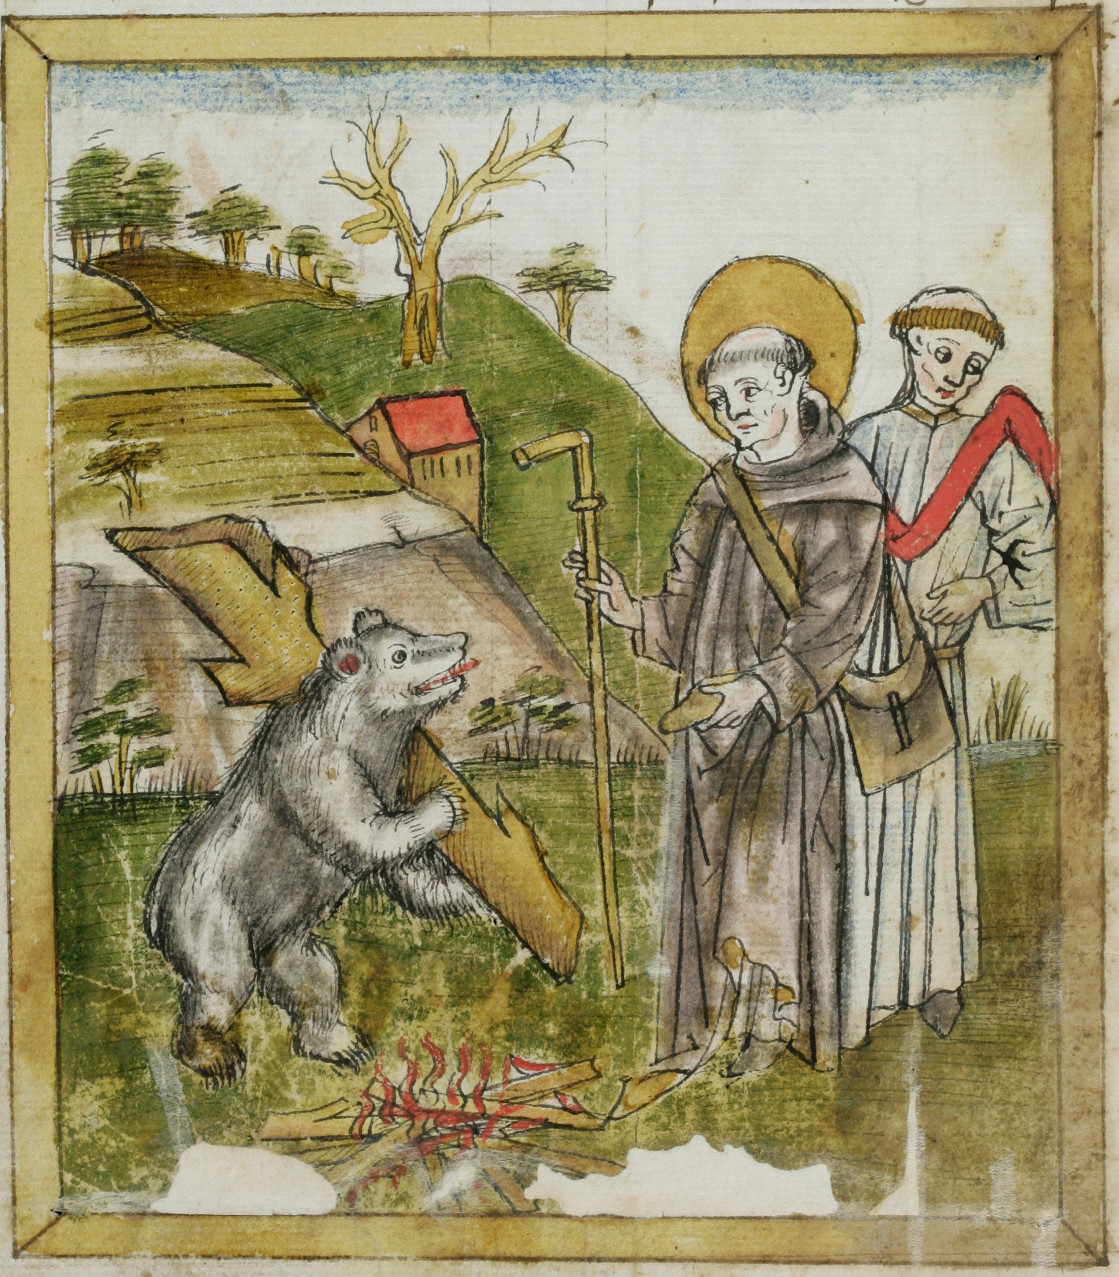
\includegraphics[width=4cm]{gallus.jpg}
\end{center}

\vfill

Fontes.
Cantus officii divini secundum
% http://www.e-codices.unifr.ch/en/sbe/0611/232v et infra
Antiphonarium pro Ecclesia Einsidlensi, Codice 611 Einsidlensi, et
% http://www.e-codices.unifr.ch/en/csg/0391/126 et infra
Antiphonarium Hartkeri, Codice 391 Sangallensi, et
Antiphonale Monasticum pro Diurnis Horis, Solesmis, 1934. /
% https://books.google.cz/books?id=j7hIAAAAcAAJ&pg=PT712#v=onepage&q&f=false et infra
Textus officii secundum Breviarium Monasterii Sancti Emmerami, Episcopi \& Martyris, pars Æstivalis,
Ratisbonæ, 1571, pag. 136 et infra, et III. nocturno lectionis secundum
% http://e-codices.unifr.ch/en/csg/0433/457/0/Sequence-542 et infra
Homiliarium, Codice 433 Sangallensi, pag. 457 et infra. /
Responsorii restituti sunt secundum interrete pagina
http://gregofacsimil.free.fr/01-Restitution/Repons/HTML/62-In-Sto-Gallo.html /
% http://e-codices.unifr.ch/en/csg/0381/455/0/Sequence-513 et infra
Sequentia secundum Versicularium, Hymnarium, Troparium, Sequentiarium,
Codice 381 Sangallensi et interrete pagina http://e-sequence.eu /
Hymnus Vita Sanctorum et antiphona ad Magnificat in I. vesperis secundum http://www.stgallerchoral.ch /
% http://www.e-codices.unifr.ch/en/bcj/0018/339/0/Sequence-66 et infra
Textus et cantus missæ secundum Graduale, Codice 18 Porrentruiensi, pag. 339,
et Graduale triplici, Solesmis, 1979. /
% http://e-codices.unifr.ch/en/csg/0359/129/0/Sequence-499 et infra
Neumæ super canto missæ supra Cantatorium, Codice 359 Sangallensi et
% http://e-codices.unifr.ch/en/sbe/0121/55/0/Sequence-974 et infra
% http://e-codices.unifr.ch/en/sbe/0121/291/0/Sequence-974 et infra
% http://e-codices.unifr.ch/en/sbe/0121/342/0/Sequence-974
Graduale \& Notkeri Sequentiale, Codice 121 Einsidlensi. /
Translatio capituli et lectionis sumpta est ex: Jeruzalémská bible, Praha-Kostelní Vydří 2009. /
Translationes psalmorum ex Hejčl Jan: Žaltář čili Kniha žalmů, Praha 1922. /

Collaborantes.
Textus latinos cantusque transcripsit et omnem laborem typographicum peregit Jakub Jelínek. /
Václav Ondráček textus hymnorum, antiphonarum, homiliarum, benedictionum
etc. in linguam bohemicam transtulit.

Instrumenta adhibita.
LuaTeX, %http://www.luatex.org /
Gregorio, %http://home.gna.org/gregorio /
typi Junicode. %http://junicode.sourceforge.net

\begin{center}
Liber hic imprimis ad usum chori
\guillemotright Conventus Choralis\guillemotleft\
paratus est
et secundum eius consuetudines.
http://www.introitus.cz

\vspace{4mm}

{\large Editio Sancti Wolfgangi \annusEditionis.}

\vspace{2mm}

Series \guillemotright Conventus\guillemotleft, vol. XII.

\vspace{4mm}

\vfill

\today

\end{center}

\end{document}
